% This must be in the first 5 lines to tell arXiv to use pdfLaTeX, which is strongly recommended.
\pdfoutput=1
% In particular, the hyperref package requires pdfLaTeX in order to break URLs across lines.

\documentclass[11pt]{article}

% Remove the "review" option to generate the final version.
\usepackage[review]{EMNLP2023}
\usepackage{multirow}
% Standard package includes d   
\usepackage{times}
\usepackage{latexsym}
\usepackage{ulem}
% \usepackage{ctex}
% For proper rendering and hyphenation of words containing Latin characters (including in bib files)
\usepackage[T1]{fontenc}
% For Vietnamese characters
% \usepackage[T5]{fontenc}
% See https://www.latex-project.org/help/documentation/encguide.pdf for other character sets

% This assumes your files are encoded as UTF8
\usepackage[utf8]{inputenc}
\usepackage{url}
% This is not strictly necessary and may be commented out.
% However, it will improve the layout of the manuscript,
% and will typically save some space.
\usepackage{microtype}

% This is also not strictly necessary and may be commented out.
% However, it will improve the aesthetics of text in
% the typewriter font.
\usepackage{inconsolata}
\usepackage{graphicx}
\usepackage{framed}
\usepackage{array}
% for subfigure
\usepackage{subcaption}
\usepackage{CJK}
\usepackage{makecell}
\usepackage[most]{tcolorbox}
\usepackage{cleveref} 
\usepackage{pifont}
% \usepackage[cmyk]{xcolor}
\newcommand{\Blue}[1]{\colorbox[RGB]{153,204,255}{#1}}
\newcommand{\Yellow}[1]{\colorbox{yellow}{#1}}
\newcommand{\Green}[1]{\textcolor[RGB]{76,153,50}{#1}}
\newcommand{\Pink}[1]{\textcolor[RGB]{210,18,150}{#1}}
\newcommand{\secref}[1]{Sec. \ref{#1}}
\newcommand{\figref}[1]{Figure \ref{#1}}
\newcommand{\eqnref}[1]{Eq. (\ref{#1})}
\newcommand{\tabref}[1]{Table \ref{#1}}
\newcommand{\exref}[1]{Example \ref{#1}}

\newcommand{\KZ}[1]{\textcolor{blue}{(Kenny: #1})}
\newcommand{\MY}[1]{\textcolor{red}{(Mengyue: #1})}
\definecolor{shadecolor}{RGB}{224, 224, 224}
\definecolor{framecolor}{RGB}{160,160,160}
% \definecolor{shadecolor}{RGB}{241, 241, 255}
% \newenvironment{prompt}
% {\begin{center}\begin{minipage}{0.9\linewidth}\begin{shaded} \small}
% {\end{shaded}\end{minipage}\end{center}\par}
\newenvironment{prompt}
{\begin{center}\begin{tcolorbox}[colback=shadecolor,%gray background
                  colframe=framecolor,% black frame colour
                  width=7.4cm,% Use 8cm total width,
                  arc=2mm, auto outer arc,
                  boxrule=0.3pt,
                 ] \small}
{\end{tcolorbox}\end{center}\par}


% If the title and author information does not fit in the area allocated, uncomment the following
%
%\setlength\titlebox{<dim>}
%
% and set <dim> to something 5cm or larger.

% \title{Leveraging ChatGPT to Power Chatbots for Psychiatric Diagnosis and Patient Simulation}
\title{LLM-empowered Chatbots for Depression Diagnosis: \\Simulation and Evaluation}
% \title{Realistic Simulation Doctor and Patients for Psychiatric Diagnosis}

% Author information can be set in various styles:
% For several authors from the same institution:
% \author{Author 1 \and ... \and Author n \\
%         Address line \\ ... \\ Address line}
% if the names do not fit well on one line use
%         Author 1 \\ {\bf Author 2} \\ ... \\ {\bf Author n} \\
% For authors from different institutions:
% \author{Author 1 \\ Address line \\  ... \\ Address line
%         \And  ... \And
%         Author n \\ Address line \\ ... \\ Address line}
% To start a separate ``row'' of authors use \AND, as in
% \author{Author 1 \\ Address line \\  ... \\ Address line
%         \AND
%         Author 2 \\ Address line \\ ... \\ Address line \And
%         Author 3 \\ Address line \\ ... \\ Address line}

\author{Siyuan Chen$^1$, Mengyue Wu$^2$\thanks{~~Corresponding Authors.}, Kenny Q. Zhu$^{3*}$,  \\ 
{\bf Kunyao Lan$^4$}, {\bf Zhiling Zhang$^5$}, {\bf Lyuchun Cui$^6$} \\
$^{1,2,3,4,5}$Shanghai Jiao Tong University, Shanghai, China \\
$^{6}$Shanghai Mental Health Center, Shanghai, China \\
\texttt{\{$^1$chensiyuan925, $^2$mengyuewu, $^4$lankunyao, $^5$blmoistawinde\}@sjtu.edu.cn,}\\
\texttt{$^3$kzhu@cs.sjtu.edu.cn, $^6$cuilvchun@outlook.com}
}


  % Affiliation / Address line 1 \\
  % Affiliation / Address line 2 \\
  % Affiliation / Address line 3 \\
  % \texttt{email@domain} \\\And
  % Second Author \\
  % Affiliation / Address line 1 \\
  % Affiliation / Address line 2 \\
  % Affiliation / Address line 3 \\
  % \texttt{email@domain} \\}

% \author{Siyuan Chen \and Mengyue Wu\thanks{~~Corresponding Authors.} \\ \and {\bf Kunyao Lan} \and {\bf Zhiling Zhang} \\ \and {\bf Minghao Lyu} \and {\bf Kenny Q. Zhu$^*$ } \\
% Shanghai Jiao Tong University \\
% Shanghai, China \\
% \texttt{\{chensiyuan925, mengyuewu, lankunyao, blmoistawinde\}@sjtu.edu.cn,}\\ 
% \texttt{qianlan844@gmail.com, kzhu@cs.sjtu.edu.cn}\\ 
% \And Lyuchun Cui \\
% Shanghai Mental Health Center\\
% Shanghai, China\\
% \texttt{cuilvchun@outlook.com}
% }


\begin{document}
\maketitle
\begin{abstract}
While using chatbots in mental health domain is receiving increasing amount of attention, implementation and evaluation of chatbots in psychiatric diagnostic scenarios remains relatively unexplored.
In this work, we focus on exploring the potential of ChatGPT in powering chatbots to simulate psychiatrist and patient for depression diagnosis. 
We collaborate with professionals to identify key objectives of such bots and iteratively develop the dialogue system to closely align with real-world scenarios. 
Additionally, we design task-specific evaluation metrics, and involve real psychiatrists and patients in diagnostic conversations with the chatbots, collecting their ratings for assessment.
Experiments shows that our doctor chatbot exhibits higher levels of empathy and diagnostic accuracy compared to the baseline; our patient chatbot can replicate human-like behaviors, including emotional fluctuations.

% \KZ{If outpatient scenarios are under-explored, then in-patient has been well studied? Shall we just say diagnotic vs.  therapeutic scenarios?}\MY{check all other  places you use``outpatient'', some can be changed into diagnostic some can just use clinical}
\end{abstract}
% COMMENT: 摘要中是不是可以简单提一下机器人诊断和模拟病人的科研或实用价值


\section{Introduction}
\label{sec:intro}

There is a growing interest in applying conversational agents (i.e., chatbots) in the mental health domain~\cite{sabour2022chatbots}. Chatbots that can (i) conduct diagnosis conversations like a psychiatrist or (ii) simulate patients in the psychiatric diagnostic scenarios, have significant real-world applications\footnote{For the sake of clarity, we will refer to these two types of chatbots as the \textbf{``doctor chatbot''} and \textbf{``patient chatbot''} respectively in the subsequent sections.}. 
Doctor chatbots can be effective tools for mental disorder screening~\cite{pacheco2021Smart} in lieu of official medical diagnosis. Patient chatbots can serve as Standard Patients (SP) in medical education, making the learning process more efficient and cost-effective~\cite{Torous2021growing}.

However, there is still limited exploration in developing and evaluating these 
chatbots, primarily due to the difficulty in obtaining dialogue data because 
of the ethical and privacy concerns for mental health issues. 
% \KZ{you just said earlier that conversational agents are increasingly being used in mental health, but now you say limited exploration. Contradictory?} 
What's more, in outpatient scenarios, depressed patients often find it difficult 
to describe their ambiguous mental state objectively, 
and they may even be ashamed or afraid of disclosing their true 
conditions~\cite{Salaheddine2016Identify}. As a result, doctor chatbots should 
go beyond serving as interactive scales (e.g., PHQ-9) for mental disorder 
screening~\cite{Yue2023Beyond}. They need to possess various professional 
skills, including emotional support, to effectively complete the diagnosis task.
Additionally, patient chatbots should resemble real patients more closely, 
rather than precisely and robotically reporting their symptoms without 
any emotional fluctuations.

\begin{figure*}[th]
	\centering
	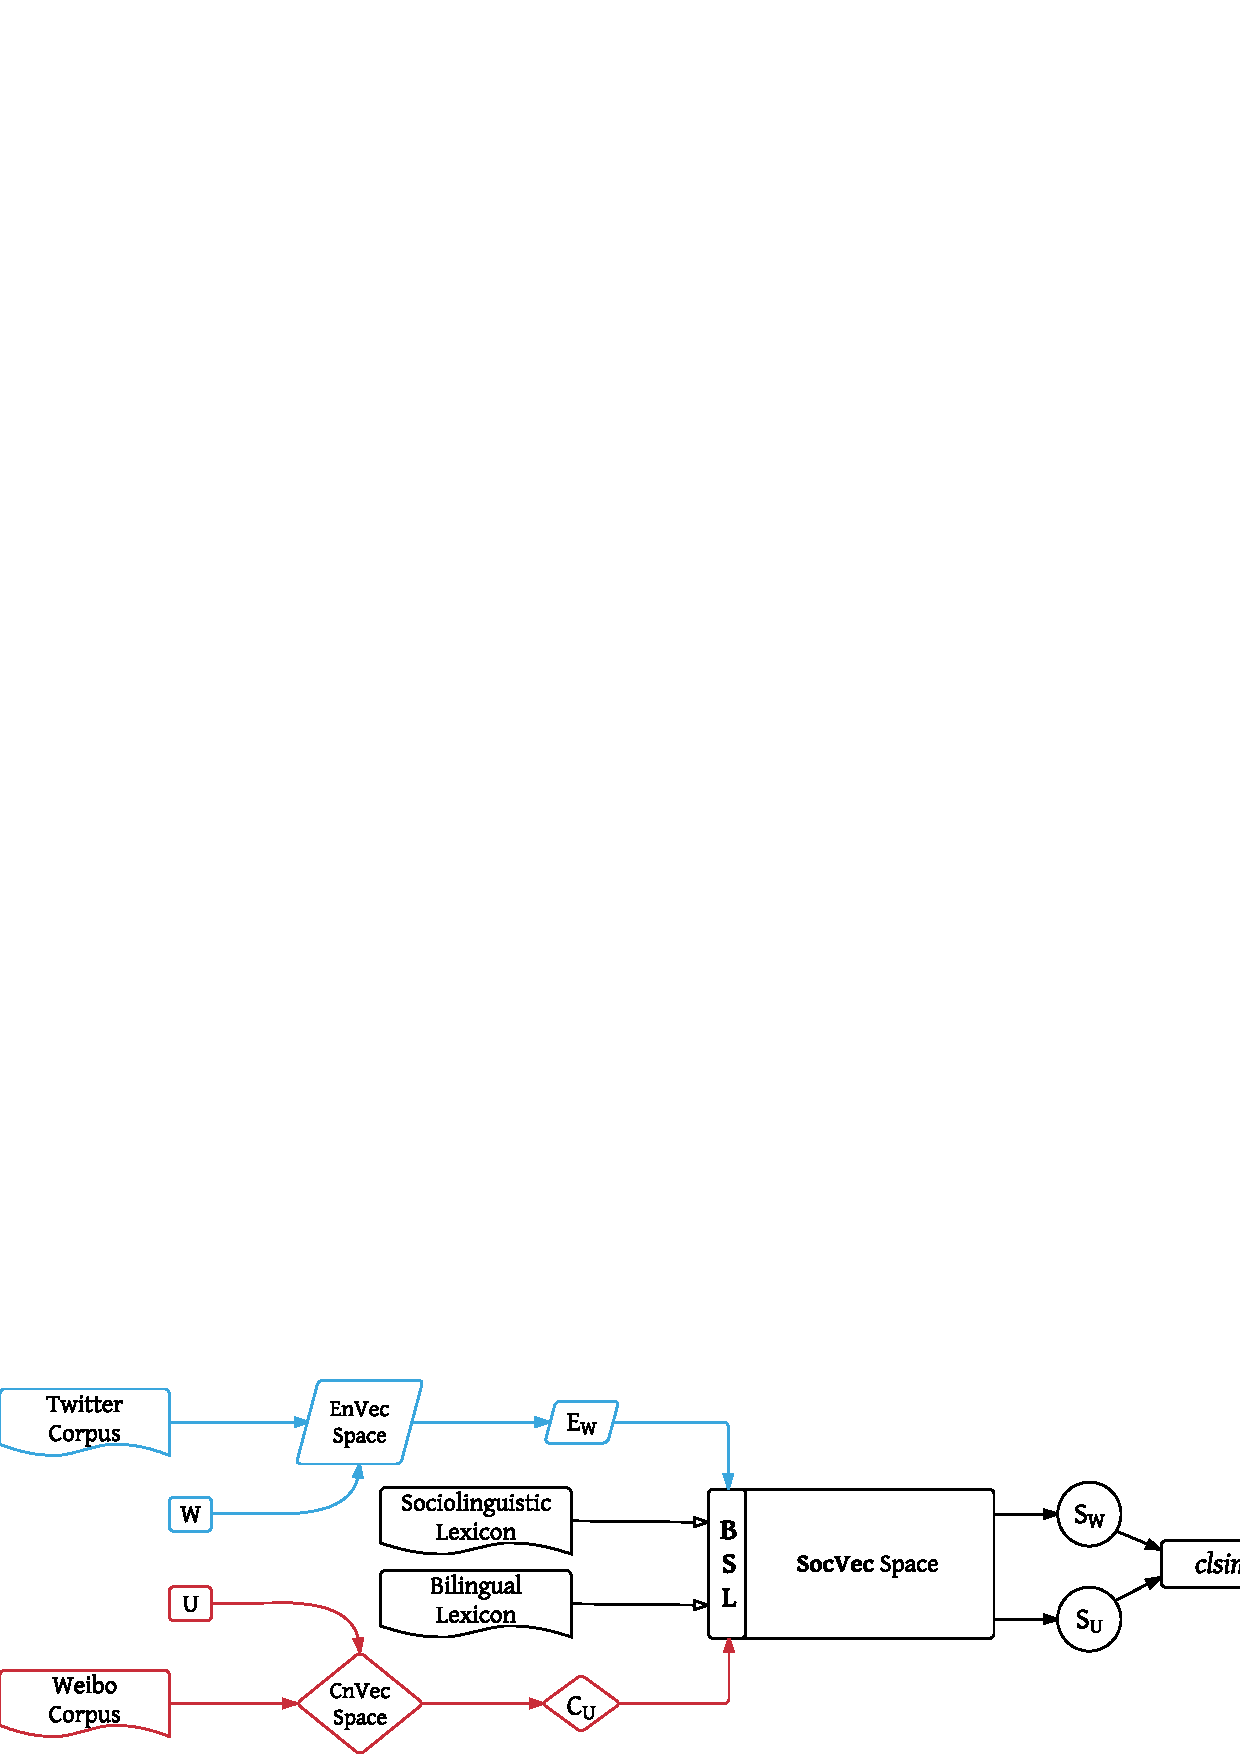
\includegraphics[width=0.8\linewidth]{Figures/overview.png}
	\caption{The overview of the expert-guided three-phase study.}
	\label{fig:pipeline}
\end{figure*}

% However, many existing frameworks~\cite{Medeiros2018UsingCF,Jaiswal2019Virtual} still rely on rule-based approaches (e.g., utilize the questions in self-rating scales), which often result in rigid conversations and cannot show sufficient empathy to patients. Alternatively, other deep learning methods \cite{yao-etal-2022-d4} require a significant amount of domain-specific data for training, which is often costly and difficult to obtain, especially in the mental health domain. 
% Furthermore, due to the diverse ways to express mental states verbally, neither rule-based nor data-based methods can comprehensively cover all possible cases, so the patient chatbots developed using these methods tend to be inflexible and lack diversity~\cite{Yao2020Toward}.

% \KZ{But how is simulating doctors and patient in diagnosis conversation more difficult than the therapeutic bots in Woebot and Wysa, and the like? In other words, why can't we use the techniques in Woebot and Wysa to simulate doctors and patients? I think the difference between diagnostic bots and therapeuric bots is that it's easier to verify quality of the doctor bot or patient bot: a good doctor bot must be able to acquire enough info efficiently from the patient so as to make a correct diagnosis; a good patient bot must resemble the real patient in doctors eyes. A good therapist however can't be easily qualified because all they are doing is to make the patient feel better, which is very subjective from the patient point of view.}  


Achieving these goals is quite difficult for conventional rule-based~\cite{Medeiros2018UsingCF,Jaiswal2019Virtual} or even data-driven~\cite{yao-etal-2022-d4, Fansi2022DDXPlus, Lin2021Graph} methods. This difficulty arises from the complexity of understanding varied human utterance in diagnosis conversations with a limited amount of pre-defined rules or training data. 
% \MY{Any reason why data-drive is not enough as well?} 
Fortunately, recent advancements in large language models (LLMs), such as ChatGPT\footnote{\url{https://chat.openai.com/}}, provide a new way to develop chatbots that can convincingly portray specific roles for its superior capability in understanding diverse natural language~\cite{Pan2023APE} and generating coherent conversations. Importantly, LLMs can achieve this with appropriate prompts rather than fine-tuning on extensive domain data.

% Equipped with comprehensive training data and knowledge, LLMs can generate diverse tones and symptom descriptions with appropriate prompts rather than fine-tuning on extensive domain data.\MY{what i meant is that why LLM can do it is not only because of its strength in generation but also understanding, these should be aligned with the challenges when using data-drive approaches}


% Achieving these goals is quite difficult for conventional rule-based~\cite{Medeiros2018UsingCF,Jaiswal2019Virtual} or even data-driven~\cite{yao-etal-2022-d4, Fansi2022DDXPlus, Lin2021Graph} methods, due to the difficulty of adequately covering complex cases of psychiatric diagnosis with a limited amount of pre-defined rules or training data. 
% % \MY{Any reason why data-drive is not enough as well?} 
% Fortunately, recent advancements in large language models (LLMs), such as ChatGPT\footnote{\url{https://chat.openai.com/}}, provide a new way to develop chatbots that can convincingly portray specific roles\MY{for its superior capability in understanding diversed natural language and generating coherant coversations, better add a ref}.  Equipped with comprehensive training data and knowledge, LLMs can generate diverse tones and symptom descriptions with appropriate prompts rather than fine-tuning on extensive domain data.\MY{what i meant is that why LLM can do it is not only because of its strength in generation but also understanding, these should be aligned with the challenges when using data-drive approaches}

% COMMENT: 前面所述,该chatbot的困难有两点:数据难采集和症状的模糊、主观。这里只讲清楚了ChatGPT能够解决数据采集的问题,那么它怎么来应对症状模糊主观的问题呢?此外还包括刚才上一段提到的,diagnosis chatbot需要提供情感支撑,patient simulator要仿真病人的情绪波动,要如何实现,这里是不是都应该简单描述一下?

Therefore, in this work, we aim to (i) respectively investigate the potential of ChatGPT in simulating \textit{psychiatrists} and depressed \textit{patients} in a clinical diagnosis scenario, 
as well as to (ii) build a comprehensive evaluation framework for these chatbots, answering the question about what constitutes a good psychiatrist chatbot and a truly patient-like chatbot.

To develop and evaluate a system that truly meets the the user's expectations, 
we follow a expert-guided design methodology. The study consists of three 
phases (See Figure~\ref{fig:pipeline}).
In \textbf{Phase 1}, as there lacks a formal description of the objectives for 
doctor and patient chatbots, we first collaborate with psychiatrists to 
identify them clearly. 
Based on these objectives, we conduct an experimental study 
(\textbf{Phase 2}) to design appropriate prompts for ChatGPT-based chatbots 
and establish an evaluation framework that incorporates both human evaluation 
and automatic evaluations aligned with the objectives from Phase 1. Importantly, the design of prompts and metrics was iterated based on human feedback, with each version improved with input from psychiatrists.
In \textbf{Phase 3}, we recruit real psychiatrists and depression patients to 
engage in diagnostic conversations with the 
simulated patient and doctor chatbots, respectively, and collect their 
ratings after conversation.
% We also conduct a comparison between the behavior of real and simulated psychiatrists based on the dialogue history, which yields some interesting findings. 

The main contributions of this work are:
\begin{itemize}
    \item We formalize the task of developing doctor and patient chatbots for depression diagnosis within an outpatient setting. In doing so, we propose specific \textit{objectives} for these chatbots that are up to near-clinical standards and establish an \textit{evaluation framework} that aligns with these objectives, with the help of practicing psychiatrists.
    \item We adopt an iterative prompt engineering approach, taking into account psychiatrists' feedback to refine the performance. By utilizing \textit{examples}, we enhance ChatGPT's understanding of professional practices. We further implement a \textit{reminder} mechanism to mitigate potential issues of forgetting when the desired behavior of chatbot being different from LLM's training purpose.
    % \MY{why is forgetting so common in our application, if it is a general phenomenon, we might want to change the reminder as patient behaviour being different from LLM's training purpose}
    \item We demonstrate the feasibility of utilizing ChatGPT-powered chatbots in mental health domain. Experiments show that ChatGPT-based doctor chatbot provides more accurate diagnostic results through more empathetic and efficient conversations with patients, comparing to the previous machine-learned chatbots.
    % \KZ{This is the first time you mention ``data-driven chatbot''. What exactly is it? Are you referring to CPT only?} 
    Moreover, the patient chatbot also exhibits emotional expression and 
resistance, which is similar to real patients. 
    % \item We suggest a data augmentation strategy that employs carefully evaluated doctor and patient chatbots to produce unlimited psychiatric outpatient dialogue data, effectively tackling the obstacle of obtaining data due to ethical concerns in mental health domain. We also provide the dataset containing dialogues between chatbots and real patients or psychiatrists from our evaluation experiments, which has been anonymized for privacy. 
    % \KZ{Ethical and privacy concerns?}
\end{itemize}




% Intuitively, relying on traditional evaluation metrics for dialogue systems (e.g., n-gram overlap, semantic textual similarity) to assess the performance of doctor and patient chatbots in mental health scenarios is inadequate, as there is no standardized answer for clinical conversations. 
% Moreover, what constitutes an exceptional psychiatrist chatbot or a realistic patient chatbot still remains unexplored. 

% Applications designed for mental health therapy or coaching in daily life, such as Woebot\footnote{\url{https://woebothealth.com}} and Wysa\footnote{\url{https://www.wysa.com}}, are gaining widespread attention for their ability to reduce users' negative emotions~\cite{Grove2021Codevelop} and promote a healthy lifestyle~\cite{Fadhil2019AssistiveCA}. Another notable application is chatbot-based symptom checkers~\cite{Yue2023Beyond}, which emulate human-like conversations while assessing users' symptoms, resembling interactive questionnaires.


\section{Objectives}
% objectives
\label{sec:objectives}
% In this paper, we ask the following scientific question:
% \begin{quote}
%     ``What constitutes a realistic doctor/patient chatbot in psychiatric outpatient conversations?'' 
% \end{quote}

Given the lack of formal definition for what constitutes a good doctor/patient chatbot in psychiatric diagnosis conversations, we invite five experienced psychiatrists to establish clear objectives and standards, which will guide us throughout the study\footnote{These psychiatrists come from top-ranked national mental health centers. 
Their professional titles and areas of expertise can be found in 
Appendix \ref{apd:psych_info}.}. 
The objectives are derived from the first two phases. In phase 1, the psychiatrists are encouraged to freely express their opinions, allowing us to summarize a set of objectives.  In phase 2, as we iteratively refine the prompts, we consult the psychiatrists for their input and identify any additional objectives to consider based on the performance of chatbot. The final objectives are organized as follows.
% \MY{how do we know that at last stage, this is the final standard? do we have a comment from doctors that the defined objectives are exhaustive and up to application standard?}

% \KZ{The following is a bit weird. Shall we change our title to include depression? Since this paper focuses on bots to diagnose depression only?}
% Considering the variation in diagnosis standards and symptoms for different mental disorders, we concentrate on depressive disorders for this study, while leaving the scaling to include other disorders as future work.

\subsection{Doctor Chatbot}
\label{sec:doc_requirements}
As a doctor chatbot, the primary task is to conduct a professional diagnostic process for the patient and provide an \textbf{accurate diagnosis}. To achieve this, a good doctor chatbot should possess the following three capacities:
% \MY{I don't think empathy-related stuff is only for user experience, it also serves the purpose of building inter-personal relation and trust for the patients, and eased their nerves for the purpose of better revealing truthful feelings and symptoms, hence a more accurate diagnosis}
\begin{itemize}
    \item \textbf{Comprehensiveness:} Inquire about the key symptoms of depression, including sleep, mood, diet, and other relevant aspects that are required for diagnosis, as defined in DSM-5~\cite{american2013diagnostic}.
    \item \textbf{In-depth Questioning:} Conduct thorough questioning (e.g., ask the duration of a symptom) based on patient's responses to gain a more precise evaluation of the symptoms.
    \item \textbf{Empathy:} Demonstrate empathy and provide emotional support to patients to establish trust and ease their nerves. This helps patients feel more comfortable in expressing their genuine feelings and symptoms, leading to a more accurate diagnosis.
    % \item Provide examples to guide patients to articulate their symptoms, rather than just asking, "Do you have any other symptoms?", the latter often causing patients to overlook important symptoms and forget to mention to the doctor.
\end{itemize}
Moreover, to offer patients superior \textbf{user experience}, the doctor chatbot should fluently switch between topics and enhance the efficiency of the conversation, thus preventing patients from feeling bored or disengaged.
\subsection{Patient Chatbot}
\label{sec:pat_requirements}

% After establishing objectives for doctor chatbots, we encountered difficulties when defining the requirements for chatbots that resemble real patients. This is due to the fact that individuals with the same disorder can exhibit significant variations in their manifestations. Moreover, psychiatrists, though experienced, have no firsthand chatting experience with a ``non-patient-like'' chatbot, making it challenging for them to generalize the requirements for a ``patient-like'' chatbot.

% To address this issue, we decide to develop an initial version of the chatbot first. This allows psychiatrists to interact with ``non-patient-like'' examples, which can help them better define the characteristics and behaviors that constitute a ``patient-like'' chatbot. Based on their feedback, we then iterate and update the chatbot accordingly.
% At this phase, we only establish one fundamental requirement for a patient chatbot.

The basic requirement for a patient chatbot is \textbf{honesty}, which entails presenting an accurate and rational description of symptoms in the provided symptom list, without reporting any non-existent ones.

Additionally, to make the chatbot more resemble real patients, psychiatrists also describe some behaviors commonly exhibited by real patients during consultations. 
\begin{itemize}
    \item \textbf{Emotion:} Patients in a depressed mental state may experience emotional fluctuations during the conversation.
    % while the chatbot's presentation of symptoms is too calm and polite. 
    \item \textbf{Expression:} Patients use colloquial expressions when describing symptoms, and may have difficulty expressing themselves clearly. They often talk about their daily life experiences. While current chatbots tend to explicitly list out the symptoms~\cite{Llanos2021Lessons} using formal language, which is too sane and professional for a patient.
    % However, the chatbot tends to use formal language similar to the official diagnostic criteria (DSM-5).
    \item \textbf{Resistance:} Patients may be reluctant to seek help. They may remain silent and refuse to communicate, or downplay their symptoms to avoid being perceived as a burden. 
    % In contrast, the chatbot is overly cooperative, readily acknowledging and providing detailed descriptions of its symptoms.
\end{itemize}




% \section{Approach}
%We first present our methods for testing short circuits in
%models, then modify some of these methods to create
%training data to reverse the short circuit problem
%and enhance the robustness of the models.
% 
%\subsection{Proxy Test for Short Circuit}
%We propose two types of approaches that can be used as proxy test for short circuits.
%One is through inspecting attention maps in
%the models under a white-box setting.
%The other is to generate new test cases by applying different operations on correct choices under a black-box setting.
%
%
%\subsubsection*{White-box Attention Weights~(AW)}
%One intuitive way to detect if an attention-based model is 
%exploiting short circuits is to visualize its attention map. 
%Given a well-trained model and a correctly answered MCQ  in the 
%form of \textit{[CLS] premise [SEP] choice [SEP]}, 
%where \textit{[CLS]} and \textit{[SEP]} are model-dependent 
%delimiters and \textit{choice} refers to the correct choice, 
%we first tokenize the input, feed the token sequence into the model, 
%and extract the attention map of all attention heads from the 
%last encoder layer.
%
%The attention maps are visualized through off-the-shelf tool~\cite{vig-2019-multiscale}
%into user-friendly demo as shown in \figref{fig:att-goodex}. 
%Human annotators are then asked to determine whether there exists 
%strong attention connections from the correct choice to the premise. 
%We consider the MCQ is solved without short-circuiting only if 
%over half of the annotators label it as having strong attention 
%connections. 
%
%Though accurate, such manual annotation is cost-prohibitive to be 
%scaled to larger tests. To remedy this issue, we propose 
%a rule-based procedure to automatically detect the short circuit 
%behavior of a model on MCQ. Specifically, we aggregate the 
%attention maps into one individual map by max-pooling over all 
%attention heads. Then we check if there exists at least one 
%attention score between token in the choice and token in the premise 
%higher than threshold $t_1$ or at least two higher than threshold 
%$t_2$, excluding special tokens like comma and period. 
%We consider that the model not short-circuiting on this MCQ if 
%neither of the two conditions is met. In practice, the 
%threshold $t_1$ and $t_2$ are tuned so as to maximally simulate 
%human annotation. The pseudo-code is shown in Algorithm \ref{AW}.
%
In this section, we first present our methods for testing short circuits in models, and then modify some of these methods to create training data to address the short circuit problem and enhance model robustness.

\subsection{Proxy Test for Short Circuit}
Since no existing method can definitively prove if a model is short-circuiting on a question, we propose two types of approaches that serve as proxy tests for short circuits. These approaches reveal the effects of model short-circuiting, though they can't directly prove the short-circuit itself, similar to dark matter. One approach involves inspecting attention maps in models under a white-box setting, while the other generates new test cases by applying different operations on correct choices under a black-box setting.

\subsubsection*{White-box Attention Weights~(AW)}

One intuitive way to detect if an attention-based model is exploiting short circuits is to visualize its attention map. Given a well-trained model and a correctly answered MCQ in the form of \textit{[CLS] premise [SEP] choice [SEP]}, where \textit{[CLS]} and \textit{[SEP]} are model-dependent delimiters and \textit{choice} refers to the correct choice, we first tokenize the input, feed the token sequence into the model, and extract the attention map of all attention heads from the last encoder layer.

The attention maps are visualized through an off-the-shelf tool~\cite{vig-2019-multiscale} into a user-friendly demo, as shown in \figref{fig:att-goodex}. Human annotators are then asked to determine whether there exists strong attention connections from the correct choice to the premise. We consider the MCQ to be solved without short-circuiting only if over half of the annotators label it as having strong attention connections.

Although accurate, such manual annotation is cost-prohibitive to be scaled to larger tests. To remedy this issue, we propose a rule-based procedure to automatically detect the short circuit behavior of a model on MCQ. Specifically, we aggregate the attention maps into one individual map by max-pooling over all attention heads. Then we check if there exists at least one attention score between a token in the choice and a token in the premise higher than threshold $t_1$, or at least two higher than threshold $t_2$, excluding special tokens like comma and period. We consider the model to not be short-circuiting on this MCQ if neither of the two conditions is met. In practice, the thresholds $t_1$ and $t_2$ are tuned to maximally simulate human annotation. The pseudo-code is shown in Algorithm \ref{AW}.


\begin{algorithm}
\small
	\caption{Attention Weight Thresholding}
	\label{AW}
\hspace*{0.02in} {\bf Input:} 
premise $P$, correct choice $C$, model $M$,  threshold $t_1$ and $t_2$. \\
\hspace*{0.02in} {\bf Output:}
binary 0/1 label $L$.
	\begin{algorithmic}[1]
		\State initialize counters $c_1$ and $c_2$ to 0.
		\State tokenize the formatted input as sequence of tokens $S$.
		\State feed $S$ into $M$ and extract the last layer's attention maps $Attn_{all}$.
		\State aggregate $Attn_{all}$ into $Attn_{max}$ by max-pooling over all attention heads.
		\For{$w_1$ in $C$}
		\For{$w_2$ in $P$}
		\If{$Attn_{max}(w_1, w_2)> t_1$}
				$c_1$ += 1
		\EndIf
		\If{$Attn_{max}(w_1, w_2) > t_2$}
				$c_2$ += 1
		\EndIf
		\EndFor
		\EndFor
		\State output 1 if $c_1>0$ or $c_2\geq 2$ and 0 otherwise.
	\end{algorithmic}
\end{algorithm}

\subsubsection*{Black-box Choice Operator}
\label{sec:proxy}
While attention-based testing methods can detect short circuits within the encoder directly, they don't directly detect short circuits in the end-to-end MCQ model, which also includes a linear layer above the attention-based pretrained language model. Additionally, these methods are limited to a family of models with inherent attention mechanisms.

A more desirable approach is an automatic end-to-end black-box test that is model-independent. In black-box testing, if a model correctly answers an MCQ, we slightly modify the MCQ by applying a certain``operation'' on the original correct choice to produce another wrong choice. The newly generated MCQ must share the same correct choice as the original question. By observing the model's response to the second MCQ, we can infer whether the model short-circuits on the original MCQ.If the model still selects the correct choice, then we consider it to have passed the test and not short-circuited on the original MCQ. The challenge now is how to construct the new wrong choice by implementing the operation in various ways.

In this paper, we consider the operations listed in \tabref{table:proxyop}. Some of the operations were mentioned in previous literature, while others are proposed here (marked with *).
The first line in each cell describes the operation, and the next two lines provide an example of constructing a false choice from a choice in the original question. An operation may either preserve (p) the truth value (\crosssymbol $\rightarrow$ \crosssymbol) or change (c) the truth value of the choice (\checksymbol $\rightarrow$ \crosssymbol).

\begin{table}[th]
        \centering
        \scriptsize
        \begin{tabular}{l|l}
                \toprule
                \textbf{Oper.} &\textbf{Description and Example}\\
                \hline
                \multirow{3}{*}{Neg+} & Add negation (c) \\
                & \textit{They called the police to come to my house. \checksymbol} \\
                & \textit{They {\color{olive}{didn't}}  called the police to come to my house. \crosssymbol} \\
                \hline
                \multirow{3}{*}{Neg-} &Remove negation (c) \\
                & \textit{Ben {\color{olive} never} starts working out. \checksymbol} \\
                & \textit{Ben starts working out. \crosssymbol}\\
                \hline

                \multirow{3}{*}{NER} &Randomly replace person names (c)\\
                 & \textit{A big wave knocked {\color{olive} Mary} down . \checksymbol} \\
                & \textit{A big wave knocked {\color{olive} Kia} down . \crosssymbol} \\
                \hline
                \multirow{3}{*}{PR*} & Switch pronoun by gender or quantity (c)\\
        &\textit{{\color{olive} She} had a great time .\checksymbol} \\
        &\textit{{\color{olive} He} had a great time . \crosssymbol} \\
                \hline
                \multirow{3}{*}{PI*} &Instantiate pronoun by randome person (c) \\
        &\textit{{\color{olive} They} gave Tom a new latte with less ice . \checksymbol}\\
        &\textit{{\color{olive} Nathanael} gave Tom a new latte with less ice . \crosssymbol}\\
                \bottomrule
%               \hline
                \multirow{3}{*}{Adv} &Add adverbs for emphasis (c) \\
                &\textit{The ocean was a calm as a bathtub .\crosssymbol} \\
                &\textit{{\color{olive} In fact} the ocean was a calm as a bathtub .\crosssymbol} \\
                \hline
               \multirow{3}{*}{CO*} & Crossover: Swap the true choices between two questions (p)\\ 
	&\textit{\color{olive}Josh got sick . \checksymbol} \\
	&\textit{\color{olive}{She had a great time .\crosssymbol}}  \\
\hline
                \multirow{3}{*}{Syn} &Replace adj/adv with synonym (p) \\
                &\textit{Dawn felt {\color{olive} happy} about getting away with it . \crosssymbol} \\
                &\textit{Dawn felt {\color{olive} glad} about getting away with it . \crosssymbol} \\

		\bottomrule
               \multirow{3}{*}{MT*} & Mutate: Swap two consecutive words (c) \\
		& \textit{Deb said yes {\color{olive} to} {\color{olive} Tim} 's marriage proposal. \crosssymbol} \\
		& \textit{Deb said yes {\color{olive} Tim} {\color{olive} to} 's marriage proposal .\crosssymbol} \\
               \hline
\multirow{3}{*}{Voice} &Swap subject and object (c) \\
        & \textit{{\color{olive}{Kara}} asked {\color{olive}{the neighbors}}  not to litter in their yard . \checksymbol} \\
        &\textit{{\color{olive}{the neighbors}} asked  {\color{olive}{Kara}}  not to litter in their yard . \crosssymbol}\\
                \bottomrule
        \end{tabular}
        \caption{A number of operations considered for proxy testing. 
First line in each cell describes the operation, the next two lines
give an example of how to construct a false choice from a choice of
the original question. An operation may either 
preserve (p) the truth value (\checksymbol $\rightarrow$ \checksymbol, \crosssymbol $\rightarrow$ \crosssymbol) or change (c) the truth value of
the choice (\checksymbol $\rightarrow$ \crosssymbol).  }
        \label{table:proxyop}
\end{table}

Inspired by boundary testing in software engineering, we can classify these operations into three equivalent classes (three vertical sections in \tabref{table:proxyop}), depending on the nature of the \textit{false} choice constructed:
\begin{enumerate}
\item The syntax and semantics are correct, and the \textit{false} choice appears similar to the \textit{true} choice.
\item The syntax and semantics are correct, and the \textit{false} choice appears distinct from the \textit{true} choice.
\item Either syntax or semantics is incorrect.
\end{enumerate}

The last class is not suitable for testing short circuits because the model may answer the proxy question correctly by eliminating the false choice due to errors in it, not by considering the premise.

We focus on perturbations on negation~\cite{checklist2020acl}, NER~\cite{checklist2020acl}, and pronouns in the first class and adverbial~\cite{wsp2020acl}, crossover, and synonym~\cite{checklist2020acl,wsp2020acl} in the second class.

While most of the operations are self-explanatory, the \textit{crossover} operation is unique and deserves special attention. Inspired by molecular biology, for each MCQ in the dataset that the model answers correctly, we substitute the original false choice with the true choice from another randomly sampled MCQ. The substituted choice remains false in the proxy question. The operation can be visually explained in \figref{fig:cross}.

\begin{figure}[th]
\centering
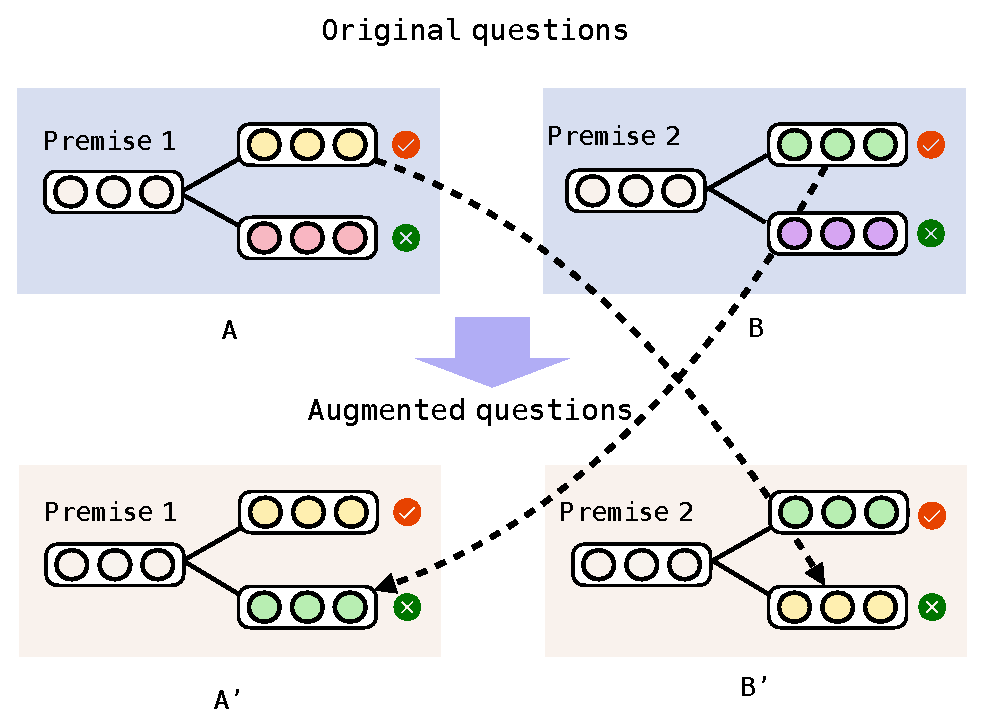
\includegraphics[width=\columnwidth]{figure/cross.eps}
\caption{The Crossover Operation: the true choice of both questions
are used to replace the false choices of these questions to create
two new proxy questions.}
\label{fig:cross}
\end{figure}

Compared to all other operations in classes 1 and 2, the crossover provides a proxy question that is most different from the original one but easier from a human perspective. This is because the two choices may be quite unrelated. If the model does not handle it correctly, it may be more indicative of a short circuit. As a result, the crossover is potentially a better short circuit test than others.

Another advantage of the crossover operation is that we can generate multiple false choices for an original question at a low cost, allowing us to test each original question more thoroughly. In contrast, most other operations cannot produce an adequate number of different variants of the original choice.

In summary, the proposed black-box choice operator provides a more generalizable and model-independent method for detecting short circuits in MCQ models. By applying various operations to create proxy questions, we can assess the model's performance and robustness more accurately, contributing to the development of better and more reliable models in the future.

\subsection{Improving Model Robustness by Data Augmentation}

If a model is shown to short-circuit by the proxy tests, its performance may decline, especially when applied to out-of-domain test data. To make models more robust, one natural thought is to generate more data to encourage models to focus on the relation between the premise and choices. While the operations used to generate proxy tests can also be utilized for data augmentation, not all of them are scalable or able to generate enough data for training.

The two operations that can generate a substantial amount of data are crossover and mutation. These operations can be applied to the training data to enhance the model's robustness.

\subsubsection*{Crossover for Data Augmentation}

Crossover is a good option for data augmentation because the two choices were originally true answers in their respective questions and presumably carry spurious features if the model was short-circuiting. By incorporating crossover into the training data, the model is forced to consider the premise in order to determine which choice is better.

\subsubsection*{Mutation for Data Augmentation}

Mutation has two flavors: (1) swap the words only in the true choice; (2) swap the words both in the true and the false choice. Compared to crossover, mutation has the potential to be more effective at improving model robustness. It not only forces the model to look into the premise due to its two very similar choices (same set of tokens), but also makes the model more sensitive to fine differences in word orders and enhances the model's prior grammatical knowledge.

\subsubsection*{Differentiating between Proxy Test and Data Augmentation}

It is essential to differentiate between the use of crossover and mutation operations in proxy tests and data augmentation. In proxy tests, these operations are used to modify the test data to assess the model's short-circuiting behavior. In contrast, when applied for data augmentation, the same operations work on the training data to enhance the model's robustness and generalization capabilities.

In conclusion, data augmentation through crossover and mutation operations can contribute to improving model robustness by encouraging models to focus on the relationship between the premise and choices. By incorporating these operations into the training data, models are forced to consider the premise and become more sensitive to the fine differences in word orders, leading to better performance and reliability in real-world applications.

\section{Prompt Design}
\label{sec:method}
% We describe the iterative methodology of designing prompts with users' feedback, which will be listed in bullet point in this section. 

% Our prompt engineering for chatbots was based on (i) the objectives proposed by psychiatrists (see Section \ref{sec:objectives}), (ii) the process of ``trial and error'', and (iii) the feedback of psychiatrists. In this part, we will discuss the design process in detail.
% \KZ{I'm assuming in the trial and error stage, you will involve
% the human doctors and patients and get their feedback. But how is this process
% actually playing out? How is it different from the final evaluation which also
% consists of human and automatic evaluation. It's a little confusing.
% I think sec 4 - 7 need to be re-organized according to the two-stage
% methodology and redesign what to put into the final evaluation section.}
% In this part, we will discuss the design process in detail.
Based on the objectives obtained in Phase 1, we started prompt engineering, which is always iterative and full of ``trial and error''.

\subsection{Design Methodology}
When designing prompts for a chatbot, it is common practice to involve humans in conversing with the chatbot for each version of the prompt. However, common applications can involve general public as human judges, while in our practice, real users (i.e., doctors and patients) are necessary to be involved to meet the requirements of real-world applications. While human engagement is essential for prompt engineering, it can also make the iterative design process time-consuming and resource-intensive.

Inspired by \citet{deriu-etal-2020-spot}, we utilize a ``bot-to-bot'' method to generate dialogue history and collect user feedback based on it. 
% \KZ{One potential issue with bot-to-bot approach, is that the initial
% version of the doc bot and patient bot must be good enough to generate
% reasonable logs.} 
Instead of the conventional ``bot-to-human'' approach, we facilitate autonomous conversations between the doctor chatbot and the patient chatbot. By leveraging this autonomous interaction, we generate dialogue history that reflects potential user interactions. These generated chat logs are then presented to real psychiatrists, who provide valuable feedback and insights based on their expertise. 
This approach allows us to simulate user interactions without requiring direct human involvement, thereby reducing the time and resources needed for the iterative design process. Moreover, we can make informed improvements and refine the chatbot in subsequent iterations by incorporating the input of healthcare professionals.

\subsection{Doctor Chatbot}
\label{sec:doc_prompt}
As illustrated in  \figref{fig:doc_prompt_design}, we undergo three iterations to develop the prompt for the doctor chatbot, and the final version is presented below:
\begin{prompt}
    \ding{192} Please play the \uline{role} of an \uline{empathetic and kind} psychiatrist. 
    \ding{193} Your \uline{task} is to conduct a professional diagnosis conversation with me based on the DSM-5 criteria. 
    \ding{194} Your questions should \uline{cover at least the following aspects}: [\ldots]\protect\footnotemark. 
    % You are free to choose the order of questions, but you must collect complete information on all aspects in the end. 
    \ding{195} Please only ask \uline{one question at a time}.
    % , and each question should only cover one symptom.
    \ding{196} You need to ask \uline{in-depth questions}, such as the \Blue{duration}, \Blue{causes} and specific \Blue{manifestations}. 
    \ding{197} You need to use various \uline{empathetic strategies}, such as \Yellow{understanding}, \Yellow{support} and \Yellow{encouragement}. 
\end{prompt}
\footnotetext{The aspects include ``emotion'', ``sleep'', etc. We provide the full list in Appendix \ref{apd:prompts}.}

\begin{figure}[th]
	\centering
	\includegraphics[width=\linewidth]{Figures/doctor_prompt_design.png}
	\caption{The iterative development process of the prompt of doctor chatbots. Psychiatrists will identify the limitations of the current version, and we will address these issues in the subsequent version.}
	\label{fig:doc_prompt_design}
\end{figure}
In this prompt, we provide a clear description of the task and establish the role to be simulated by the doctor chatbot. Then, we list the specific aspects that the doctor chatbot should cover during the questioning process. This serves as a guideline to ensure the \textit{comprehensiveness} objective. What's more, we include examples (highlighted in colored boxes) in the prompt to guide the doctor chatbot in asking \textit{in-depth} questions and demonstrating \textit{empathy}. These examples are crucial because, without them, the chatbot tends to ask superficial questions and  rely on generic phrases like ``thank you very much for your answer'' to show empathy. This arises from ChatGPT's limited comprehension of ``in-depth questioning'' and ``empathy'' in clinical contexts. Consequently, providing examples can be a promising approach to help ChatGPT grasp certain specialized skills within professional domains.

\subsection{Patient Chatbot}
\label{sec:pat_prompt}
After two iterations, we arrive at the final version of the prompt for the patient chatbot, which is presented below:
\begin{prompt}
    \ding{192} Please play the \uline{role} of a patient, who is currently chatting with a doctor. 
    \ding{193} \uline{You are experiencing the following symptoms}: [\texttt{Symptom List}]\protect\footnotemark 
     % \KZ{Instead of giving the full list of symptoms in the prompt, shouldn't we give a random subset of those symptoms?}
    \ding{194} Please talk to me based on the above symptom list. 
    \ding{195} You can only mention \uline{one symptom per round}. 
    \ding{196} You should \Blue{express} your symptoms in a \uline{vague and colloquial} way, and relate them to your \uline{life experiences}.
    \ding{197} You can have \Blue{emotional fluctuations} during the conversation. 
    \ding{198} You have a \Blue{resistance} towards doctors, and do not want to reveal some feelings easily.
\end{prompt}
\footnotetext{The symptom list is summarized by ChatGPT and revised by psychiatrists. See Appendix \ref{apd:symp_list} for details.}

In the first iteration, we describe the task (sentence \ding{192}\ding{193}), provide a symptom list (sentence \ding{194}) in the prompt, and add sentence \ding{195} to avoid listing all the symptoms in one turn. 
This prompt enables the chatbot to meet the basic requirement of providing \textit{honest} responses in most cases.
However, feedback from psychiatrists indicates that the chatbot lacks resemblance to real patients as it does not effectively convey \textit{emotions}, use colloquial \textit{expressions}, or demonstrate \textit{resistance} to seeking help. 

Therefore, we add sentence \ding{196}, \ding{197}, \ding{198} to address these issues in the second iteration.
However, we observe that the effect of adding these sentences is most prominent in the initial rounds of conversation, suggesting that the patient chatbot tends to forget some of the instructions given at the beginning. 
This behavior is reasonable considering ChatGPT's training objective to be a helpful, polite AI assistant that provides detailed responses. Consequently, there can be a potential mismatch between the desired behavior of the patient chatbot, including resistance and emotional fluctuations, and the training objective, making it more likely for these instructions to be forgotten.

To address this issue, we insert new reminders during the conversation. Inspired by the fact that the latter part of the prompt has the greatest impact on the responses generated by ChatGPT, our method is straightforward yet effective. Without users' awareness, we covertly append the following words at the end of the most recent sentence in the dialogue history.

\begin{prompt}
    (\Yellow{Attention:} colloquial language, life experience, low mood or mood swings, refuse or answer briefly due to resistance)
\end{prompt}

We aim to use simple phrases or words as reminders during the conversation to ensure that the sentences are not overly long. Moreover, these reminders are only temporarily attached to the most recent round, and will not persist in the dialogue history for subsequent rounds.
% With these reminders, the patient chatbot can maintain a colloquial language style consistently and exhibit resistance even in the latter part of the conversation, so we consider this version as the final one\footnote{The final version is in Table \ref{tab:patient_prompt} in Appendix \ref{apd:prompts}.}.


\section{Evaluation Framework}
\label{sec:eval_frameworks}
% \KZ{Are we only evaluating the final version of the two bots from prev section? This is not part of the iterative design process right? This should be made clearer.}
% \MY{normally we provide objective/automatic eva first, followed by human evaluation results. when introducing the metrics and results, follow this order}

Guided by psychiatrists and through an iterative development process, we established the objectives for two chatbots and completed their designs in Phase 2. In addition, we also designed an evaluation framework, which will be employed in Phase 3 to assess the performance of the developed chatbots. This section will describe our evaluation framework which encompasses interactive experiments for human evaluation and various task-specific metrics.
\subsection{Chatbots of Comparison}
% \KZ{this section should go into the evaluation framework?}

Due to the complexity and high time cost of human evaluation, we select several representative prompt versions for comparison, and discuss the evaluation process of doctor and patient chatbots respectively.

\paragraph{Doctor Chatbot} 
Each patient will have a conversation with four different doctor chatbots in a random order, and then rate them on four human evaluation metrics with 1-4 scale. 
Three of the chatbots are powered by ChatGPT. \texttt{D1} uses the full prompt, 
while the other two (i.e., \texttt{D2}, 
\texttt{D3}) have certain parts removed for ablation. 
The fourth chatbot, \texttt{CPT}, is a representative deep learning chatbot trained on domain-specific data \cite{yao-etal-2022-d4} using CPT model~\cite{shao2021cpt}. 
% \MY{Make a table for these bots, including doctor and patient}
\paragraph{Patient Chatbot}
Each psychiatrist will have a conversation with two patient chatbots, and then rate their performance with 1-4 scale. 
The two patient chatbots are \texttt{P1} and \texttt{P2}, aligning with the prompt versions in Section \ref{sec:pat_prompt}. 
A brief description of these chatbots can be found in Table \ref{tab:cmp_chatbots}.
% The first one uses the full prompt while the second one omits additional parts for realistic in version 2\footnote{Detailed description and prompt of these doctor/patient chatbots are shown in Appendix \ref{apd:prompts}.}.
% COMMENT: 这两段要引述一下表1啊。此外1中的"xx parts"的表述,最好和前面一致,都用v1v2v3或者①②③这种方式来提,更容易理解。CPT这个模型的名字也应该在正文里写出来。

\begin{table}[h]
    \centering
    \footnotesize
    \begin{tabular}{m{0.1\columnwidth}|c|m{0.6\columnwidth}}
    \hline
    & Chatbot & Description \\
    \hline
    \multirow{4}{0.1\columnwidth}{Doctor} & D1 & use the full doctor prompt \\
    \cline{2-3}
    & D2 & remove empathy parts in prompt  \\
    \cline{2-3}
    & D3 &  remove aspect part in prompt \\
    \cline{2-3}
    & CPT & CPT model trained on domain data \\
    \hline
    \multirow{2}{0.1\columnwidth}{Patient} & P1 & use the prompt in the first iteration \\
    \cline{2-3}
    & P2 & use the full patient prompt\\
    \hline
    \end{tabular}
    \caption{Brief description of the chatbots for comparison. Detailed description and prompt is in Appendix \ref{apd:prompts}.}
    \label{tab:cmp_chatbots}
\end{table}
\subsection{Evaluation Metrics}
\label{sec:eval_metric}
When designing evaluation metrics, our goal is to ensure that each objective is accompanied by appropriate metrics for accurate measurement.  We employ both human and automatic metrics for evaluation, and divide the automatic metrics of both kind of chatbots into two types: \textbf{function} and \textbf{style}. The overview of these metrics and their relations to objectives can be found in \figref{fig:all_metric}.
% \MY{Clearer now, but still mixing function and style - which objectives and metrics are function-related and which are style?}.
% NEWCOMMENT: 这里这样分类之后,在图中也要把两类指标区分出来,可以在objective那一列上做区分
\begin{figure}[th]
	\centering
	\includegraphics[width=\linewidth]{Figures/metrics.png}
	\caption{The correspondence between evaluation metrics and objectives. \textbf{\textit{Function}} metrics are orange, and \textbf{\textit{style}} metrics are gray.}
	\label{fig:all_metric}
\end{figure}

\subsubsection{Metrics for Doctor Chatbot}
\label{sec:doc_metric}
\paragraph{Human evaluation} In most cases, patients do not have specialized knowledge in psychiatry, making it difficult for them to assess a doctor's professional skills precisely. Therefore, when designing human evaluation metrics for doctor chatbots, we focus mainly on the user experience. The metrics are shown in Table \ref{tab:human_eval_doctor}.
\begin{table}[h]
    \centering
    \footnotesize
    \begin{tabular}{m{0.18\columnwidth}|m{0.7\columnwidth}}
    \hline
    Metrics & Explanation \\
    \hline
    Fluency & The chatbot does not repeat previously asked questions and can smoothly switch between different topics. \\
    \hline
    Empathy & The chatbot can understand and comfort you properly. \\
    \hline
    Expertise & The chatbot behaves like a real doctor, making you believe in its professionalism. \\
    \hline
    Engagement & The chatbot can maintain your attention and make you want to continue talking to it. \\
    \hline
    \end{tabular}
    \caption{Human evaluation metrics of doctor chatbot.}
    \label{tab:human_eval_doctor}
\end{table}
\paragraph{Automatic evaluation}
Different from human evaluation metrics, we mainly measure the expertise of the doctor chatbot using automatic metrics. 
The \textit{functional} requirements for doctor chatbot is to provide an accurate diagnosis, so the corresponding metric is \uline{``diagnosis accuracy''}. 
The \textit{style} part concerns the doctor chatbot's professional skills. We use \uline{``symptom recall''} to evaluate the chatbot's ability to comprehensively gather the patient's symptom-related information, and use \uline{``in-depth ratio''} to assess the ability to ask in-depth questions for deeper understanding. 
To ensure a better user experience, we calculate the \uline{``average number of questions''} asked in a single interaction to discourage the chatbot from overwhelming patients with excessive queries. Furthermore, we employ the metric of \uline{``symptom precision''} to penalize the chatbot's mechanistic behavior of asking all potential questions, irrespective of the user's responses. 

\subsubsection{Metrics for Patient Chatbot}
\label{sec:pat_metric}
\paragraph{Human evaluation}
There is no standard to measure whether a patient is ``good'' enough. Thus, when chatting with patient chatbots, doctors can only assess whether their style of expression and manner of communication resemble real patients enough and whether they can describe their symptoms in a reasonable way, so the main metrics for human evaluation are \textbf{Resemblance} and \textbf{Rationality}.
What's more, we divide the Resemblance metric into three aspects in Table \ref{tab:human_eval_patient}, according to the objectives in Section \ref{sec:objectives}.

\begin{table}[h]
    \centering
    \footnotesize
    \begin{tabular}{m{0.18\columnwidth}|m{0.65\columnwidth}}
    \hline
    Metrics & Explanation \\
    \hline
    Mental State & The chatbot is in depressed state, such as be in low mood, reluctance to communicate, scattered thoughts, etc.\\
    \hline
    Life Experience & The description of symptoms is related to daily life and personal experiences.\\
    \hline
    Language Style & Use colloquial and natural expressions when describing symptoms.\\
    \hline
    \end{tabular}
    \caption{Three aspects of the ``Resemblance'' metric.}
    \label{tab:human_eval_patient}
\end{table}
\paragraph{Automatic evaluation}
The \textit{functional} requirement of patient chatbot is ``honesty'', and we can calculate \uline{``wrong symptom ratio''} by comparing the patient's symptom list with the symptoms it reported to assess this aspect. 

Then, we evaluate the patient chatbots' \textit{style} using some linguistic features, like \uline{``Human/robot-like word ratio''}, to find out whether their language is colloquial with limited usage of professional terminology. We also use \uline{``unmentioned symptom ratio''} to measure the resistance level of chatbots. 

\subsubsection{Computation and Annotation}
A detailed explanation of the automatic metrics for the doctor and patient chatbot can be found in Appendix \ref{apd:eval}. 
In addition, to calculate some of these metrics, we need to annotate the dialogue history. This involves identifying the relevant symptom in the doctor's question, determining whether the patient truly experiencing a certain symptom, and so on, which is described in Appendix \ref{apd:annotation}.
Due to the inadequacy of dialogue history data for training multiple classification models, we employ ChatGPT to automatically label each sentence in the dialogue history, leveraging its impressive annotation capabilities~\cite{Gilardi2023ChatGPTOC}. Subsequently, three annotators thoroughly review and rectify the results to ensure the quality of the annotation.
% To assess the performance of dialogue systems, it is crucial to employ both human evaluation and automatic metrics, especially in mental health domain. Since there is little previous work on how to evaluate simulated psychiatrists and patients, we design several task-specific metrics and interactive experiments for human evaluation. 

\subsection{Human Evaluation Participants}
% We first implemented a website to host our chatbots, making it easier for participants to interact with them and rate their performance. The details of the website can be found in Appendix \ref{sec:chatInterface}. 
%\subsubsection{Participants}
In contrast to the approach of using actors/actresses to simulate patients as mentioned in \citet{yao-etal-2022-d4}, our evaluation process involves actual depression patients and psychiatrists, enabling us to assess the performance of chatbots in real-world scenarios.

Depression patients are recruited through online advertisements.
A total of 14 volunteers completed the entire process, with ages ranging from 18 to 31, and male and female participants accounted for 28.57\% and 71.43\% respectively. 
To assess the severity of their depression, patients are asked to complete the Beck Depression Inventory~\cite{beck1996beck}. Notably, we have a balanced distribution of healthy, mild, moderate and severe depression subjects which distribution is presented in Table \ref{tab:distribution_seve} in Appendix \ref{apd:eval}.
% \KZ{If the severity is ``none'', this patient is considered healthy?}

We invited 9 psychiatrists who are not involved in the prompt design, through cooperation with hospitals. Two of them are graduate students majoring in psychiatry, and the rest are practicing psychiatrists with rich clinical experience to ensure the professionalism of the evaluation.
% \footnote{Detailed information about these psychiatrists is in Appendix.}. 
% \KZ{Better provide anonimized version of their affiliations in the appendix, to make these people more credible?} \MY{Agree with Kenny's comment here, we can include their affiliation and how many years of expertise in this field}




% To ensure the quality of the dialogue data and evaluation, we also utilize a series of quality control strategies, which can be found in Appendix \ref{apd:quality}.


% COMMENT: 自动评测是如何实现的,如何自动把“症状”和“诊断结果”从对话中抽取出来,应该需要在这里说明一下



\subsection{Experimental Setup}
\label{sec:preprocess}
In this paper, we use Probase\cite{WuLWZ12} and WordNet\cite{wordnet}
as two alternative isA taxonomies. Probase is a large collection of
concept-subconcept or concept-entity pairs which were
extracted automatically by the Hearst pattern\cite{Hearst92} from
a large web corpus. Because this knowledge base is harnessed from large
data, it contains statistical scores of the extracted pairs,
such as the popularity,
and the conditional probability between the concept and its sub-concept.
WordNet, on the other hand, is a smaller, cleaner knowledge base manually
curated by experts and does not contain any scoring information.
These two taxonomies provide two different vocabularies of concepts
from which to draw the solution of AC.
%Our primary target of verb is a set of 200 most frequently used verbs in
%English text\footnote{We compute the frequency of all verbs that appeared
%in a very large web text corpus to obtain the 200 most frequently used
%verbs. We excluded a few verbs such as ``use'', ``make'', ``get'' and
%``take'' from the top of the list because they are extremely general and
%have too many arguments.},
%which we call Verb-200. These verbs are shown in \figref{fig:verbs}. A random
%sample of 20 verbs from Verb-200 forms a smaller set of verbs called Verb-20
%(highlighted in \figref{fig:verbs}) which are used in most of our experiments.

All our experiments are based on two large
datasets\footnote{We release most of
our datasets and the action concept lexicon at
\url{http://adapt.seiee.sjtu.edu.cn/~kzhu/ac}.}
from Web sentences (called Web for short) and
Google syntactic N-gram data\cite{goldberg2013,googlengram}
(called Google for short), respectively.
The 3734 most frequently used verbs (including verb phrases)
in the Web data form a primary verb set called {\bf Verb-3734}.
A subset of 2323 verbs that can be found in the Google dataset
form another verb set called {\bf Verb-2323}.
%We compute the frequency of all verbs that appeared
%in a very large web text corpus to obtain the 3734 most frequently used
%verbs.
A random sample of 20 verbs from the 200 most frequently
used verbs form the smallest set of verbs called {\bf Verb-20}
(in \figref{fig:verb20}), %which are used in most of our experiments.
which are used in some of the experiments.

The Web dataset contains 49,911,718 verb-subject pairs
and 65,035,827 verb-object pairs extracted from 165,758,215 English
sentences, which is a crawled snapshot of web pages.
%\KZ{How many subject-verb pairs and verb-object pairs in web data?}
%\KZ{How many?}\textcolor{red}{[KQ:We don't know...]}
%in a snapshot of Bing's search log.
The Google dataset contains
32,731,395 verb-subject pairs and 43,580,062 verb-object pairs
from the \emph{Verbargs} package, which includes 130,436,458
syntactic N-grams.% with verb-argument dependencies.
%\KZ{How many subject-verb pairs and verb-object pairs in google data?}
%\KZ{Kaiqi: We need to describe how we generate the web and
%google data sets here.
%Need to emphasize how big these data sets. Remember this ``VL''DB!}

\begin{figure}[th]
\centering
\fbox{\parbox{.8\columnwidth}{
bring,
carry,
connect,
cut,
define,
eat,
help,
hit,
keep,
operate,
perform,
play,
read,
release,
report,
select,
spend,
submit,
visit,
wear
}}
\caption{Verbs in Verb-20}
\label{fig:verb20}
\end{figure}

ReVerb also provides millions of relation triples, some of which contain
verbs as predicate.
%However, the scale of ReVerb is small to our problem.
We aim at discovering the action concepts,
which needs a large number of action instances
for each verb. However, ReVerb contains small number of triples for each verb.
For example, only 374 unique triples for ``wear'' are
extracted in ReVerb while our web dataset contains 17,749 unique
\pair{verb}{object} pairs for ``wear''.
The reason of the huge different is that,
a triple must contain two arguments for the verb in ReVerb. However,
verbs co-occur with only one argument in many cases.
Moreover, ReVerb has little coverage on
intransitive verbs, which only come with subject.
We give up using ReVerb data due to these limitations.
%\KZ{We need to explain why we don't use the ReVerb data.}

%\subsection{Preprocessing of Dataset}
%To make use of the web sentences and Google syntactic N-gram,
Next, we preprocess the two datasets as follows to
generate action instances.

{\bf Web} data comes from the result of Stanford dependency parser,
%We run a dependency parser on the whole corpus and
which are dependency trees for the sentences. We are interested in
verb-subject and verb-object relations only.
The head word of subject is usually labeled
as ``nsubj'' or ``agent'' while the head word of object is usually
labeled as ``dobj'' or ``nsubjpass''.
We can retrieve the entire phrase of subject or object in the dependency
tree by returning the whole subtree rooted on the head.
However, the whole phrase of subject/object is not always
a term recognizable by the taxonomies. As shown in \figref{fig:pterm},
the phrase ``a flashy baseball cap''
is extracted as the object of ``wear'', but 
it is not a valid Probase/WordNet term.
To make use of the taxonomies, we need to
detect the Probase/WordNet term from the subject/object phrase
(e.g., baseball cap).

\begin{figure}[th]
\centering
\epsfig{file=pterm.eps,width=0.8\columnwidth}
\caption{Dependency Parse Tree}
\label{fig:pterm}
\end{figure}

We use a sliding window strategy to extract longest
Probase/WordNet term that we can detect in the whole phrase.
The window slides around the head word
from right to left, and check if a Probase/WordNet term exists.
The initial size of the window is the length of the
whole phrase. If we detect a Probase/WordNet term,
we return the phrase captured in the window;
Otherwise, we decrease the window size and slides
around the head term again. We stop until we find
any Probase/WordNet term. Usually, this procedure can detect
a Probase/WordNet term from the phrase, because Probase/WordNet includes
most of the words (phrase with length 1). After
preprocessing, we output all the pairs of verb-subject and
verb-object as action instances.
%\begin{table}[th]
%\centering
%%\scriptsize
%\caption{Snapshot of Google Syntactic N-gram}
%\begin{tabular}{|l|l|}
%\hline
%Verb & N-gram \\
%\hline \hline
%accept & firms/NNS/nsubj/2\; accept/VBP/conj/0\; \\
%& money/NN/dobj/2\; in/IN/prep/2\; \\
%& exchange/NN/pobj/4   \\
%\hline
%delay & to/TO/aux/2\; delay/VB/xcomp/0\; \\
%& these/DT/det/4\; matters/NNS/dobj/2 \\
%\hline
%spent & an/DT/det/2\; afternoon/NN/nsubjpass/4\; \\
%& was/VBD/aux/4\; spent/VBN/conj/0\\
%\hline
%\end{tabular}
%\label{tab:ngram}
%\end{table}

\textbf{Google} data contains relations between
verbs and arguments.
%A snapshot
%of Google syntactic n-gram is shown in \tabref{tab:ngram}.
%The syntactic n-gram consist of the dependency parsing
%result conducted by Stanford parser.
Each token is labeled with POS tag, dependency and head index.
To apply this data to our task,
we restore each n-gram to a dependency tree according
to the head index and 
adopt the same processing as in Web to extract 
pairs of \pair{verb}{subject} and \pair{verb}{object}.
%First, we restore each n-gram to a dependency tree
%according to the head index. Next, we find the head of the
%subject or object from the nodes that directly connects to
%the verb node with a dependency label such as ``nsubj'', ``agent'', ``dobj''
%or ``nsubjpass''. Around the head, we use the same sliding window
%algorithm to find a longest Probase/WordNet term to be the subject/object
%as in the processing of the web data. Also, we convert
%the verb to its lemma form.
%After this process, we finally get two lists of pairs
%in the form of \pair{verb}{subject} and \pair{verb}{object}, respectively.

The subsequent experiments are conducted on lexicons learned from
different combinations of verb sets, taxonomies and datasets. For
readers' convenience, the configurations of these experiments are documented
in \tabref{tab:comb}.
\begin{table}[th]
\centering
%\scriptsize
\caption{Verbs, taxonomies and datasets for each experiment}
\begin{tabular}{|l|c|c|c|}
\hline
Experiment & Verb Sets & Taxonomies & Datasets \\
\hline \hline
Accuracy \& Overlap & Verb-20 & Probase &  Web, Google\\
\hline
\multirow{2}{*}{Execution Times} & Verb-3734, & Probase,
	& \multirow{2}{*}{Web, Google} \\
	& Verb-2323 & WordNet & \\
\hline
Verb Sense Matching & Verb-3734 & WordNet & Web \\
\hline
Argument Identification & Verb-20 & Probase & Web \\
\hline
WSD & Verb-3734 & WordNet & Web \\
\hline
Verb Frame Generation & Verb-3734 & Probase & Web \\
\hline
Term Similarity & Verb-3734 & Probase & Web \\
\hline
\end{tabular}
\label{tab:comb}
\end{table}

%\begin{figure}[th]
%\centering
%\fbox{\parbox{2\columnwidth}{
%\sout{use
%make
%include
%take
%get
%provide
%show}
%go
%say
%find
%see
%come
%work
%need
%look
%require
%give
%{\bf help}
%offer
%know
%create
%change
%add
%start
%allow
%{\bf keep}
%{\bf play}
%contain
%run
%apply
%receive
%call
%develop
%leave
%begin
%hold
%support
%cause
%build
%meet
%increase
%cover
%base
%want
%serve
%continue
%{\bf read}
%write
%produce
%{\bf bring}
%involve
%pay
%live
%ask
%put
%consider
%set
%reduce
%remove
%improve
%appear
%{\bf perform}
%seem
%move
%lead
%follow
%buy
%occur
%try
%design
%contact
%complete
%sell
%learn
%determine
%think
%{\bf report}
%describe
%like
%present
%mean
%relate
%lose
%feel
%affect
%post
%represent
%enjoy
%send
%open
%discuss
%{\bf visit}
%enter
%grow
%share
%maintain
%identify
%indicate
%tell
%place
%list
%return
%choose
%{\bf select}
%turn
%sign-up
%form
%obtain
%stop
%check
%result
%win
%happen
%install
%{\bf wear}
%die
%love
%understand
%save
%expect
%focus
%fill
%watch
%prevent
%{\bf spend}
%protect
%reach
%pass
%raise
%display
%treat
%ensure
%{\bf connect}
%achieve
%establish
%suggest
%view
%accept
%associate
%fit
%drive
%exist
%control
%talk
%replace
%deliver
%avoid
%hear
%fall
%let
%{\bf define}
%handle
%{\bf eat}
%plan
%bear
%prepare
%manage
%{\bf release}
%promote
%attend
%experience
%join
%kill
%seek
%{\bf operate}
%measure
%end
%refer
%teach
%face
%conduct
%explain
%purchase
%combine
%test
%{\bf cut}
%generate
%review
%deal
%break
%close
%reflect
%decide
%believe
%consist
%{\bf carry}
%fail
%collect
%speak
%address
%encourage
%match
%stand
%sit
%stay
%{\bf hit}
%{\bf submit}
%draw
%walk
%depend
%limit
%please
%reveal
%introduce
%wait
%arrive
%enable
%}}
%\caption{Verb-200 (Ranked) with Verb-20 in Bold}
%\label{fig:verbs}
%\end{figure}

%bring\\
%carry\\
%connect\\
%cut\\
%define\\
%eat\\
%help\\
%hit\\
%keep\\
%operate\\
%perform\\
%play\\
%read\\
%release\\
%report\\
%select\\
%spend\\
%submit\\
%visit\\
%wear\\
%\hline
%\end{tabular}
%\label{tab:verbs}
%\end{table}
%



\section{Experiments}
\label{sec:experiments}
In this section, we conduct
extensive experiments on slogan generation 
to evaluate the performance
of the proposed model SALE.
We introduce the dataset, 
the competing models and parameter settings,
as well as the evaluation metrics.
We also demonstrate the experimental results in a series of evaluations
and perform further analyses on the effectiveness of our approach
in generating accurate, fluent, informative and attractive slogans.

\subsection{Dataset}
\label{sec:dataset}
We first introduce the text corpora we create
for slogan generation task in e-commerce.
Then we describe the evaluation dataset we used in
our following experiments.
The datasets are released at \url{https://202.120.38.146/slogan/}.

\subsubsection{Dataset for Slogan Generation}
\label{sec:corpora}
%In this section, we describe the experimental setup,
%especially the hyper-parameter configurations of 
%the Seq2Seq framework we used in following experiments. 
%We also detail dataset used in our experiments.
Slogan generation in E-commerce is a relative new problem.
Thus, there is a lack of dataset for this task.
We created a new dataset, containing 
the basic information of the topics attending to potential focuses or selling-points,
including the topic and its item preference, as well as the slogan.
The data are collected from Taobao, a large-scale website for e-commerce in China.

We use the pattern of ``\emph{PV} + \emph{CG}" 
to construct topics from frequent phrases mining from largely amount
of query logs and product titles.
The product titles are composed by the sellers and content producers on the
website.
We construct multiple item preferences for each topic by sampling items from 
secondary categories as well as human intervention to 
make the items with an item preference concentrate more on a specific focus 
or selling-point.
Thus, in each instance, a topic is annotated with an item preference semi-automatically
by leveraging the category ontology introduced in \secref{sec:introduction}.
Then, we recruit experts to write a slogan for each data instance.
Overall, the dataset contains 857 topics and 
in total 3,555 $(x, p, y)$ instances after preprocessing.

We use four splits named (train/dev/LMdev/test) in our experiments.
Note that, the LMdev split is for 
hyper-parameter $\beta$ tuning (see \secref{sec:shallow_fusion} in details).
The splits are randomly divided based on topics 
proportionally by 90\%, 5\%, 1.5\% and 3.5\%.
Thus each split of (train/dev/LMdev/test) includes 771, 43, 13, 30 topics separately,
and correspond to 3132 training instances, 231 development instances, 
50 LM development instances, as well as 142 test instances.

%For the evaluation dataset, 
\subsubsection{Evaluation Dataset}
\label{sec:eval_dataset}
We perform algorithm evaluation and human evaluation
in our experiments (see \secref{sec:metrics} in details).
Thus we provide two evaluation datasets separately for each.
We directly use all the 142 instances of test split in \secref{sec:corpora},
referred as FULLtest,
for the algorithm evaluation which are based on automatic scoring systems,
such as BLEU.
Besides, we randomly sample 50 instances from the test split
to form a small evaluation dataset for human evaluation,
referred as HUMtest.


\subsection{Compared Methods}
\label{sec:compared}
In this section, we introduce the baseline and choices for 
our model components, as well as the parameter settings
used in those models.

\subsubsection{Baselines and SALE}
\label{sec:baselines}
According to the problem statement (in \secref{sec:problem})
and the proposed item preference fusion methods (in \secref{sec:preference}),
the models for comparison backed by Seq2Seq framework are mainly one-way input models and two-way input models.

One-way input models (prefixed by \emph{One}) takes in one-way input as the source sequence,
and the slogan as its target sequence, without considering 
semantics enhancement or incorporating pretrained language model.
There are three one-way input baselines with different inputs.
\textbf{One-T} (\textbf{t}opic) model
takes the topic itself as its source sequence,
while \textbf{One-P} (item \textbf{p}reference) model takes
the titles of items as its source sequence.
Then, 
%while 
\textbf{One-CAT} (con\textbf{cat}nating) model 
concatenates the topic and its item preference with special token \emph{SEP}
as a separator, and takes the sequence of concatenation as its source sequence.

The two-way input models (prefixed by \emph{Two})
are designed to treat topics and item preferences heterogeneously.
We propose two kinds of two-way input models
based on different heterogeneous inputs fusion methods 
(see details in~\secref{sec:preference}).
%we propose two fusion methods in \secref{sec:preference}
%to combine the heterogeneous inputs.
\textbf{Two-BiAttn} (\textbf{bi}directional \textbf{att}ending) model use the two-way bidirectional attending
to combine the representations of topics and that of item preferences.
\textbf{Two-CAT} (con\textbf{cat}nating) model use two-way concatenating strategy 
to fuse the heterogeneous outputs of encoders.

For \textbf{SALE}, 
we incorporate the semantics enhancement module
(in \secref{sec:semantics}) to enrich
the deep contextualized representations
backed by Two-CAT baseline.
\textbf{SALE+PLM} integrates
%On the basis of SALE, 
%we integrate
pre-trained language model (PLM) 
into SALE at inference time in order to improve
the generalization and robustness of the model.
%Specially, SALE identifies the \emph{is-a} relations
%among heterogeneous inputs and
%increase the semantic capacity of the model for better contextualized representations
%knowledge-aware module

\subsubsection{Parameter Settings}
We use an architecture of 8 stacked convolutional layers 
for both the topic encoder and the item preference encoder
as well as the decoder parts with kernel width as 3.
To enable deep convolutional networks, 
we add residual connections~\cite{he2016deep} from the input of each convolution
to the output of the layer as well.
For each convolutional layer, we set the hidden vector size as 512
and the embedding size as 256.
To alleviate the overfitting problem, we add the dropout ($p=0.2$)
layer~\cite{srivastava2014dropout} for all convolutional layers and fully connected layers.

To optimize the proposed models,
we use Nesterov's accelerated gradient method
~\cite{sutskever2013importance} with gradient clipping 0.1
~\cite{pascanu2013difficulty},
momentum 0.99, and 
learning rate 0.2.
We terminate the training process when the learning rate drops 
below 10e-5.
We set beam size as 5 for the beam search algorithm
in the testing step.
The hyper-parameter $\beta$ of SALE-PLM (in ~\eqnref{eq:shallow_fusion})
was selected to maximize the generation performance
on the LMdev split by grid search, from the range 1e-4 and 0.1.


\subsection{Evaluation Metrics}
\label{sec:metrics}
We perform both algorithm evaluation and human evaluation
in our experiments.
Specially, we evaluate our model on generation quality which includes
the automatic scoring metrics such as
BLEU and lexical diversity,
as well as a number of human-evaluation metrics.

\paragraph{BLEU}
The BLEU algorithm~\cite{papineni2002bleu} compares consecutive phrases of the 
generated slogan with the consecutive phrases it finds
in the reference slogan, and counts the number of matches, in a weighted fashion.
A higher BLEU score indicates a higher degree of similarity with the reference
slogan.
We compare all competing models on test split in terms of the BLEU score as a sanity check.
We also use BLEU score as the standard metric to finetune
hyper-parameter $\beta$ in SALE+PLM model.

\paragraph{Lexical Diversity}
A common problem in automatic text generation is that the system tends to generate safe
answers with enough diversity~\cite{li2016deep}.
A low diversity score often means generated contents are general and vague, 
while higher diversity means the generated contents are more informative and 
interesting.
Following~\cite{ChenLZYZ019}, we calculate the number of distinct n-grams produced on the test split
as the measurement of the diversity of generated descriptions.

\paragraph{Human-evaluation Metrics}
Automatic scoring metrics including BLEU score and lexical diversity are competitive and inexpensive to operate.
However, they do not consider
other important aspects such as intelligibility and grammatical correctness (or fluency) of slogan.
We use several human-evaluation metrics
to evaluate competing models on various perspectives.
\begin{itemize}
	\item \textbf{Overall quality} is designed to measure the
	overall generation quality of model.
	\item \textbf{Relevancy} is used to measure the content relevancy of generated slogan to the given topic and items.
	\item \textbf{Fluency} focus on the intelligibility and grammatical correctness of generated slogan.
	\item \textbf{Interestingness} takes personification and attractiveness into account.
\end{itemize}


\subsection{Performance Comparisons and Analysis}
\label{sec:results}


In this section, we conduct an analysis of our proposed model
to evaluate the contribution of item preference fusion module and
semantics enhancement module as well as the integration of 
pre-trained language model.

We evaluate competing models on FULLtest and HUMtest 
as we described in \secref{sec:eval_dataset}.
The comparison results of slogan generation are shown in 
\tabref{tab:auto_eval} and \tabref{tab:human_eval}.
For human evaluation, we recruit three experts as annotators 
and ask them to give scores on each aspect of generated slogan, 
range from 1 to 5,
then average the scores of each aspect on HUMtest as 
human evaluation results.


\begin{table*}[th]
	%	\small
	\centering
	\caption{Slogan generation results comparison with baseline methods using FULLtest.}
	\label{tab:auto_eval}
	\begin{tabular}{lcccc}
		\hline
		Model %& Overall quality 
		& BLEU &  Diversity (n=2) ($\times 10^2$ )& Diversity (n=3) ($\times 10^2$ ) & Diversity (n=4) ($\times 10^2$ ) \\
		\hline
		One-T %&  3.30  
		&  28.34 &  2.25   &  2.45  &  2.37 \\
		One-P %&  3.86  
		&  41.11 &   4.74 &    5.99 & 6.33 \\
		One-CAT  % & 3.82  
		& 38.86  &  3.86 &  4.77  & 4.94 \\
		Two-BiAttn  % & 3.86  
		& 36.99  &  4.82 &  5.87  &  6.03   \\
		Two-CAT % & 3.95
		& 40.59  &  4.89 &  5.99  &  6.22 \\
		\hline\hline
		SALE % & \textbf{4.16}  
		& 42.31  & 4.87  &  6.20 &  6.55  \\
		SALE+PLM % & -  
		& \textbf{42.36}   &  \textbf{4.89} & \textbf{6.23}  &  \textbf{6.57}  \\
		%		SingleSG$_{\mathrm{concept}}$ & 28.34 &  3.30 & 3.32 & 4.31 & 4.38 \\
		%		SingleSG$_{\mathrm{items}}$& 41.11 & 3.84 & 4.0 & 4.30 & 4.22  \\
		%		MultiSG-{biattn} & 36.99 & 3.86 & 4.05 & 4.17 & 4.11 \\
		%		MultiSG-{cat} & 40.59 & 3.95 & 4.13 & 4.34 & 4.23  \\
		\hline 
	\end{tabular}
\end{table*}



\begin{table}[th]
	\small
	\centering
	\caption{Human evaluation for slogan generation task using HUMtest.}
	\label{tab:human_eval}
	\begin{tabular}{lcccc}
		\hline
		Model & Overall quality & Relevancy &  Fluency & Interestingness \\
		\hline
		One-T &  3.30  &  3.32 &  4.31   &  4.38 \\
		One-P &  3.84 &  4.0 &   4.30 &    4.22  \\
		One-CAT  &  3.62  & 3.94  & 4.24  & 4.18  \\
		Two-BiAttn  & 3.86  & 4.05  &  4.16  &  4.11     \\
		Two-CAT & 3.95  & 4.13  &  4.34 &  4.23   \\
		\hline\hline
		SALE & \textbf{4.16}  & \textbf{4.32}  & \textbf{4.53}  &  \textbf{4.43}  \\
		SALE+PLM & -  & -   &  - &   -  \\
		%		SingleSG$_{\mathrm{concept}}$ & 28.34 &  3.30 & 3.32 & 4.31 & 4.38 \\
		%		SingleSG$_{\mathrm{items}}$& 41.11 & 3.84 & 4.0 & 4.30 & 4.22  \\
		%		MultiSG-{biattn} & 36.99 & 3.86 & 4.05 & 4.17 & 4.11 \\
		%		MultiSG-{cat} & 40.59 & 3.95 & 4.13 & 4.34 & 4.23  \\
		\hline 
	\end{tabular}
\end{table}



Firstly, we show the importance of item preference for  slogan generation.
We introduce item preference features for specific topic
using category ontology as discussed in \secref{sec:preference}.
Topic and its item reference are simply concatenate into one input sequence
in One-CAT model. 
As we can see that One-CAT substantially outperforms One-T which only use topic as input
with an advantage of +0.32 overall quality (relatively 9.7\%), +10.5 BLEU, +110.7\% diversity ($n=2$), +144\% diversity ($n=3$) and +81\% diversity ($n=4$),
Thus, item preference plays an important role in slogan generation task.

However, the results show that
One-P model which only takes in item preference as input outperforms
One-CAT on various metrics.
This imposes that topic and item preference are two heterogeneous inputs,
thus we should treat them differently in the model using item preference fusion method.
Next, we analyze the contribution of item preference fusion methods proposed
in \secref{sec:preference}
by comparing One-CAT, Two-BiAttn and Two-CAT.
We can see that show that two-way concatenating method for Two-CAT
substantially outperforms two-way directional attending for Two-BiAttn.
Though Two-CAT model slightly decreases on BLEU compared to One-P,
Two-CAT outperforms One-P according to human evaluation shown in \tabref{tab:human_eval}.
This suggests that two-way bidirectional attending fusion 
makes the semantics corruption between two heterogeneously deep contextualized representations.
Therefore, two-way concatenating fusion method is more effective for 
heterogeneous inputs combination.

Our proposed \emph{is-a} knowledge-aware model SALE 
is backed by Two-CAT, equipping with the semantics enhancement module.
Results show the effectiveness of semantics enhancement module
proposed in \secref{sec:semantics}.
As shown in \tabref{tab:human_eval} and \tabref{tab:auto_eval}, 
SALE outperforms Two-CAT by a substantial margin.
Specially, semantics enhancement improves the
diversity scores ($n=3, 4$) 3.5\%, 5.3\% separately .
SALE also achieves an improvement of 1.72 (relatively 4.24\%) in terms of BLEU, 
as well as an improvement of 0.57 in terms of overall quality.
We can see that SALE outperforms all previous baselines on every aspect.
Thus SALE is able to generate accurate, fluency, informative and attractive slogans.
We further illustrate this in \secref{sec:cases}. 



Lastly, we analyze the contribution of pre-trained language model integration
comparing results of SALE and SALE+PLM.
As shown in \tabref{tab:auto_eval}, 
incorporating PLM at inference stably improves the diversity 
that performs best at every n-gram diversity scores ($n=2,3,4$).
Note that, we finetuned hyper-parameter $\beta$ for SALE+PLM 
in terms of BLEU score on LMdev split,
and SALE+PLM with $\beta = 2e\mathrm{-}4$ achieves best BLEU score as 42.94.
Thus, we use $\beta=2e\mathrm{-}4$ for SALE+PLM model in test.
As shown in \tabref{tab:auto_eval}, SALE+PLM 
outperforms all competing models in terms of BLEU score as 42.36 
on FULLtest dataset.
Since the results generated by SALE and SALE+PLM are nearly the same on HUMtest,
their human evaluation results are same, 
we do not show result of SALE+PLM in \tabref{tab:human_eval}.
We can see that in this case the improvement of PLM integration is minor but stable, 
on both BLEU score and diversity scores.
We argue that such PLM integration makes our model more robust.

% the contribution of item preferences in one-way input models: OneT, OneP, OneCAT
% item preference fusion methods for two-way input models: OneCAT, Two-BiAttn, Two-CAT
% is-a knowledge-aware model SALE: Two-CAT, SALE, SALE+PLM




\subsection{Case Studies}
\label{sec:cases}
In this section, we perform case studies to observe 
how our propose methods influence the generation so that
the model can generate different slogans for a specific topic
according to different item preferences.
Besides, our proposed \emph{is-a} knowledge-aware model SALE generate higher quality slogans
benefiting from semantics enhancement.

%The running example in \tabref{sec:introduction} illustrates 

In \tabref{tab:vary_preference}, % \tabref{tab:vary_preference}
two item preferences are provided for topic ``早教玩具" (early education toys).
The first preference consists of musical toys such as ``音乐拍拍鼓" (musical patting drum),
which focuses on music education for children,
while the second preference is mainly about ``手摇铃" (rattle) which focuses on improving concentration ability 
as well as soothe emotions for babies.
The second example of 
\tabref{tab:vary_preference} is the running example we discussed in \secref{sec:introduction}.
The proposed model SALE successfully captures those focuses 
and generate attractive slogans accordingly.
For example, SALE generates \emph{music enlightenment}
for the focus of musical patting drum
and generates \emph{soothe baby's emotion } for the focus of 
rattle.
As shown in \tabref{tab:vary_preference}, 
we use red color to mark the preferences and its effects for slogan generation.

We also demonstrate the effectiveness of semantics enhancement
by comparing slogans generated by SALE and Two-CAT in \tabref{tab:semantics}.
%as shown in \tabref{tab:semantics}.
\tabref{tab:semantics_a} shows two example topics associated with an item preference each.
The entities involved in \emph{is-a} relations
have been marked as blue. 
The third column of \tabref{tab:semantics_a} demonstrates the 
identified relations.
\tabref{tab:semantics_b} compares slogans generated by SALE and Two-CAT
for the topics in \tabref{tab:semantics_a}.
Results show that SALE enhanced by \emph{is-a} knowledge 
tends to integrate the inferred user needs into slogan,
for example \emph{the first choice when preparing a gift for mom} for ``large size mother-dress"
and \emph{always protect you} for ``outdoor sports protective gear",
which further promotes user interests.


%\KZ{You need to translate these into English.}
% Please add the following required packages to your document preamble:
% \usepackage{multirow}
\begin{table*}[th!]
\begin{center}
\caption{Two examples of generated slogans by the proposed model SALE, varying
	the item preference while fixing the topic as input.}
\label{tab:vary_preference}
\small
%\subfloat[Example of slogans generated by SALE.]{
%	\label{tab:vary_preference_a}
		\begin{tabular}{c|c|c}
		\hline
%		\multicolumn{1}{c}{topic}  
		topic                                                                    
		& item preference                   
%		& semantic relations                                                                                                                    
		& slogan                                                                         
		\\ \hline
		\multirow{2}{*}{\begin{tabular}[l]{@{}l@{}} \\ 早 教 玩 具 \\ early education toys\end{tabular}} 
		& \begin{tabular}[l]{p{65mm}l@{}}
%			澳 贝 青 蛙 小 鼓 音 乐 手 拍 鼓\\ (ao bei frog)\\ 
			儿 童 益 智 早 教 玩 具 宝 宝 \color{red}{音 乐 拍 拍 鼓} \\ 
			intelligence early childhood education toys \quad 
			\color{red}{musical patting drum for baby}
%			\\ 宝 宝 音 乐 拍 拍 鼓 儿 童 益 智 电 动 玩 具 \\ (译文)
		\end{tabular} 
		& \begin{tabular}[l]{p{65mm}l@{}}
		    \textcolor{red}{音 乐} \color{black}{早 教} \color{red}{启 蒙} , 
			\color{black}{宝 宝 智 能 } \color{red}{手 拍 鼓} \\ 
			early childhood education \quad \color{red}{music} \quad \color{red}{enlightenment}
			\textcolor{black}{, intelligent} \quad \color{red}{patting drum} \quad
			\color{black}{for baby} 
		\end{tabular} \\ \cline{2-3} 
		& \begin{tabular}[l]{p{65mm}l@{}} 宝 宝 益 智 早 教 婴 幼 儿 \color{red}{手 摇 铃} \\
			\textcolor{red}{rattle} \color{black}{for baby intelligence early education}
%			\\ 澳 贝 新 生 婴 儿 牙 胶 手 摇 铃\\ (译文) 
		\end{tabular}            
%		& \begin{tabular}[c]{@{}l@{}}
%			手 拍 鼓, \emph{hypo}, 玩 具
%		\end{tabular}                                                    
		& \begin{tabular}[l]{p{65mm}l@{}}婴 儿 益 智 \color{red}{摇 铃}, \color{red}{安 抚} \color{black}{宝 宝} \color{red}{情 绪} 
			\color{black}{神 器}\\ intelligence development \color{red}{rattle} 
			\color{black}{for baby, the best tool to} \color{red}{soothe} \color{black}{the baby}
		\end{tabular}    \\ \hline
%	\end{tabular}
%}
%\cut{%%%%%%%%%%%%
%\qquad
%\subfloat[]{
%	\label{tab:vary_preference_b}
%	\begin{tabular}{c|c|c}
%		\hline
		%		\multicolumn{1}{c}{topic}  
%		topic                                                                    
%		& item preference                   
%		%		& semantic relations                                                                                                                    
%		& slogan                                                                         
%		\\ \hline
		\multirow{2}{*}{\begin{tabular}[l]{@{}l@{}} \\ 玻 璃 灯 具\\ glass light fixture \end{tabular}} 
		& \begin{tabular}[l]{p{65mm}l@{}}客 厅 \color{red}{ 现 代 简 约 吸 顶 灯} \color{black}{两 室 一 厅 套 装 灯} \\ 
			\textcolor{red}{morden style living room ceiling light} \quad light set for two-bedroom apartment
%			\\ 创 意 led 客 厅 吸 顶 灯 水 晶 灯 \\ (译文)
		\end{tabular} 
		& \begin{tabular}[l]{p{65mm}l@{}}\textcolor{red}{现 代} \color{black}{元 素} \color{red}{吸 顶 灯} , 彰 显 \color{red}{极 简} 魅 力 \\ 
		\textcolor{red}{ceiling lights} \color{black}{in} \textcolor{red}{modern} \color{black}{style, shining} \textcolor{red}{minimalist} \color{black}{charm} 
		\end{tabular} \\ \cline{2-3}
		& \begin{tabular}[l]{p{65mm}l@{}}
%			台 灯 卧 室 床 头 灯 温 馨 浪 漫 ins 少 女 个 性 创 意 \\(译文) \\ 
			钟 爱 一 生 台 灯 卧 室 \color{red}{暖 光} \color{black}{床 头 灯} \color{red}{温 馨} \color{black}{布 艺} \\ 
			the favorite table lamp \quad table lamp with \color{red}{warm ligth} \color{black}{for living room} \quad \color{red}{warm} \color{black}{cloth art}
		\end{tabular}            
		& \begin{tabular}[l]{p{65mm}l@{}} 一 灯 一 世 界, 一 亮 一 \color{red}{温 馨} \\ 
		lights in your world, bright and \textcolor{red}{warm}  
		\end{tabular} \\ \hline
	\end{tabular}
%    }%%%%%%%%%%
%}
\end{center}
\end{table*}


\begin{table*}[th!]
	\begin{center}
		\caption{The influence of semantics enhancement for slogan generation.}
		\label{tab:semantics}
		\small
		\subfloat[Examples of relation identification in SALE.]{
			\label{tab:semantics_a}
			\begin{tabular}{c|c|c}
				\hline
				%		\multicolumn{1}{c}{topic}  
				topic                                                                    
				& item preference       
				%		& semantic relations                                                                                                                    
				& semantic relations                                                                         
				\\ \hline
				\begin{tabular}{p{10em}}
				大 码 \color{blue}{妈 妈 装 }\\ large size \color{blue}{mother-dress}
				\end{tabular}
				& \begin{tabular}{p{20em}}
				中 老 年 \color{blue}{女 装} \color{black}{秋 装 长 袖 连 衣 裙 夏 中 年 妈 妈 装 打 底 衫 秋 春 季 大 码 连 衣 裙 子} \\ middle-aged and old \color{blue}{women's clothing} \quad \color{black}{autumn long sleeves \quad summer dress  \quad blouses for middled-aged women  \quad large size dresses for spring and autumn
				}   \end{tabular} 
				& \begin{tabular}{p{12em}<{\centering}} (女 装, \emph{hyper}, 妈 妈 装)  \\ (women's clothing, \emph{hyper}, mother-dress ) \end{tabular} \\ 
				\hline
				
				\begin{tabular}{p{10em}}
					户 外 运 动 \color{blue}{ 护 具 }\\ outdoor sports \color{blue}{protective gear}
				\end{tabular}
				& \begin{tabular}{p{20em}}
					裤 袜 加 长 \color{blue}{护 小 腿 } \color{black}{超 薄 跑 步 健 身 } \color{blue}{护 膝} \color{black}{护 具 男 女 运 动 装 备}   \\
					lengthen legging pantyhose \quad \color{blue}{leg protector} \quad \color{black}{ultra thin sports} \color{blue}{knee pads} \quad \color{black}{sports protective gear for men and women} 
				\end{tabular} 
				& \begin{tabular}{p{12em}<{\centering}} (护 小 腿, \emph{hypo}, 护 具)  \\ (leg protector, \emph{hypo}, protective gear) \\
				 (护 膝, \emph{hypo}, 护 具) \\ (knee pad, \emph{hypo} protective gear) \end{tabular} \\ 
			    \hline
				
			\end{tabular}
		}
	\qquad
		\subfloat[Comparision of capturing potential user needs.]{
		\label{tab:semantics_b}
		\begin{tabular}{c|c}
			\hline  
			model                                     & slogans                           \\ \hline
			\begin{tabular}{p{7em}<{\centering}}Two-CAT\end{tabular}
			& \begin{tabular}{p{32em}} 中 老 年 连 衣 裙 , 时 尚 \\ 
			middle-aged and old women's dress, fashion\end{tabular} \\ 
			\begin{tabular}{p{12em}<{\centering}}SALE\end{tabular}	
			& \begin{tabular}{p{32em}} 中 老 年 连 衣 裙 , \color{blue}{送 妈 妈}  \color{black}{的 首 选}\\
			middle-aged and old women's dress, the best choice \color{blue}{for mommy}
		 \end{tabular} \\ 
			\hline
			\begin{tabular}{p{7em}<{\centering}}Two-CAT\end{tabular}
			& \begin{tabular}{p{32em}} 运 动 套 装 , 穿 出 潮 流 感 \\ 
			sports sweatsuit, fashion \end{tabular} \\ 
			\begin{tabular}{p{12em}<{\centering}}SALE\end{tabular}	
			& \begin{tabular}{p{32em}} 运 动 不 能 少 , 时 刻 \color{blue}{保 护} 你 \\ 
			exercise is indispensable, \color{blue}{protecting} \color{black}{you at all time}
			\end{tabular} \\ 
			\hline
			
		\end{tabular}
	}

	\end{center}
\end{table*}
%大 码 妈 妈 装
%中 老 年 女 装 秋 装 长 袖 连 衣 裙 夏 中 年 妈 妈 装 打 底 衫 秋 春 季 大 码 连 衣 裙 子
%中 老 年 连 衣 裙 , 送 妈 妈 的 首 选
%中 老 年 连 衣 裙 , 时 尚 时 尚
%
%户 外 运 动 护 具
%篮 球 骑 行 登 山 健 身 护 腿
%裤 袜 加 长 护 小 腿 超 薄 跑 步 健 身 护 膝 护 具 男 女 运 动 装 备
%运 动 套 装 , 穿 出 潮 流 感
%运 动 不 能 少 , 时 刻 保 护 你

%玻 璃 灯 具
%
%(glass light fixture)
%
%欧 式 吸 顶 灯 圆 形 LED 吸 顶 灯 具
%创 意 led 客 厅 吸 顶 灯 水 晶 灯


%音 乐 早 教 启 蒙 , 宝 宝 智 能 手 拍 鼓
%
%(译文)
%
%儿 童 安 抚 摇 铃 , 哄 娃 益 智 两 手 齐 抓
%
%(译文)


%儿 童 早 教
%
%(early childhood education)
%
%
%澳 贝 青 蛙 小 鼓 音 乐 手 拍 鼓,
%(译文)
%儿 童 益 智 早 教 玩 具 澳 贝 宝 宝 音 乐 拍 拍 鼓
%(译文)
%宝 宝 音 乐 拍 拍 鼓 儿 童 益 智 电 动 玩 具 
%(译文)
%
%
%音 乐 早 教 启 蒙 , 宝 宝 智 能 手 拍 鼓 
%(译文)



% Please add the following required packages to your document preamble:
% \usepackage{multirow}

%\begin{table*}[th!]
%\begin{center}
%\caption{Study cases for generated slogans.}
%\label{tab:vary_preference}
%\subfloat[Each pair of slogans is generated by varying the item preference while fixing the topic as input. ]{
%        \label{tab:case_a}
%\begin{tabular}{p{1.5em}<{\centering}|p{27em}|p{5em}}
%	\hline
%	\multicolumn{1}{c}{\multirow{2}{*}{topic: 儿 童 早 教 \\ (early childrenhood education)} }
%
%	\hline
%	\end{tabular}
%}
%\end{center}
%\end{table*}

%\caption{Each pair of slogans is generated by varying the item preference while fixing the topic as input. }

%长 袖 大 码 妈 妈 装
%
%儿 童 玩 具
%宝 宝 巴 士 正 品 奇 奇 妙 妙 形 象 熊 猫 公 仔 宝 宝 的 好 伙 伴 礼 物 娃 娃 毛 绒 玩 具
%
%儿 童 玩 具 , 玩 出 百 变 造 型
%创 意 玩 具 , 捏 出 百 变 造 型
%
% 1 2 个 月 儿 童 早 教
% 宝 宝 手 拍 鼓 , 早 教 益 智 好 伙 伴
% 音 乐 早 教 启 蒙 , 宝 宝 智 能 手 拍 鼓
% 儿 童 早 教 益 智 玩 具 清 单
% 益 智 音 乐 玩 具 , 开 发 宝 宝 无 限 智 力


\section{Conclusion}
We implement a novel sequence-based dependency parsing
framework which takes advantage of high order features 
in parsing history. 
%We can also adapt beam search to this framework so as to
%relax the strictly greedy nature. Vine pruning\cite{rush2012vine} could
%be incorporated to speed up the parsing.
More importantly, we discovered that the parsing accuracy is very sensitive to
the quality of parsing sequence. Future work can be focused on
developing better sequence predictors that outperform Malt action classifier.
Furthermore, we use two sets of features for sequence predictor and
head mapper right now. A unified set of features between these two components
are worth exploring.
%Besides, better sequence predicting method and unified feature
%representation of two components are worth exploring.
%
%Though we currently get a not bad result,
%the sequence predictor still needs more exploration.
%According to our experiment, slightly changes
%on the sequence can lead to a fatal decline on accuracy. Ensuring the match degree of training sequence and testing
%sequence demands a high quality of sequence predictor.
%
%Further, the features in our current implementation are not expanded and well tuned yet  and we are free to define high order features to make use of parsing history. Our framework is flexible to merge other technics to enhance the performance. Introducing beam could make up for our greedy decoder and improve our accuracy. Vine pruning\cite{rush2012vine} could speed up parsing process. Besides, better sequence predicting method and unified feature representation of two components are worth exploring.

\section*{Ethics Statement}

\paragraph{Annotation} We pay the annotators a fair wage above the minimum requirement.
If workers have any questions or concerns, we will respond to them immediately. 
Since the content involves the expression of mental disease symptoms, we may expect negative effects on the annotators. Therefore, the annotators can freely take breaks or quit the task at anytime. 
We also interviewed some annotators about their feeling after annotation. They only reported slight discomfort at the time of reading sad or frightening posts due to empathy, and they found no long-term negative effects on them.

\paragraph{Application} Mental disease detection can be related to some sensitive topics, so we should be careful with its applications. First, since mental diseases like depression are still not well understood or even stigmatized in many regions, improper usage of MDD techniques may do harm to the users. Moreover, the precision and recall of the algorithm is far from prefect. It may make false/missing diagnoses which can prevent the user from getting proper treatment, but may still be an useful auxiliary tool for those who are unaware of their mental conditions or cannot access mental services. Therefore, the predictions of the model should be carefully re-examined by professionals for a confirmed diagnosis, where the symptom prediction results may facilitate quick inspection when served as the disease-specific summary of the long posting history. 
We will also require the users of PsySym to comply with a data usage agreement to prevent the invasion of privacy or other potential misuses. 

\section*{Limitation}

The discovery of dog sound units heavily relies on the quality of the dataset. 
Even though we have implemented multiple measures to enhance the dataset's quality, noise may still be present due to various factors, including the recording equipment, background noise, or added noise by video uploaders. 
Further research may focus on finetune PANNs or other sound event detection models to acquire datasets of higher quality.

% Additionally, \XY{TODO: the limitation of word discovery}


% Entries for the entire Anthology, followed by custom entries
\bibliography{anthology,custom}
\bibliographystyle{acl_natbib}

\appendix

\begin{table*}[th]
    \centering
    \tiny
    \resizebox{\linewidth}{!}{
        \begin{tabular}{cccccccc}
        \hline
        \textbf{Case} & \textbf{Character} & \textbf{Initial} & \textbf{Final} & \textbf{Rule} & \textbf{Initial IPA} \\
        \hline
        direct                      & \begin{CJK*}{UTF8}{gbsn}波\end{CJK*} &  \begin{CJK*}{UTF8}{gbsn}帮\end{CJK*} & \begin{CJK*}{UTF8}{gbsn}戈\end{CJK*} & \begin{CJK*}{UTF8}{gbsn}帮\end{CJK*}=[p] and \begin{CJK*}{UTF8}{gbsn}戈\end{CJK*}=[\textipa{uA}] & [p] \\
        \multirow{2}{*}{rule-based} 
        & \begin{CJK*}{UTF8}{gbsn}砩\end{CJK*} & \begin{CJK*}{UTF8}{gbsn}帮\end{CJK*} & \begin{CJK*}{UTF8}{gbsn}废\end{CJK*} & \multirow{2}{*}{if(initial=\begin{CJK*}{UTF8}{gbsn}帮\end{CJK*} and final=\begin{CJK*}{UTF8}{gbsn}废\end{CJK*}) then [f] else [p]} & [f] \\
        & \begin{CJK*}{UTF8}{gbsn}碑\end{CJK*} & \begin{CJK*}{UTF8}{gbsn}帮\end{CJK*} & \begin{CJK*}{UTF8}{gbsn}支\end{CJK*} &  & [p] \\
        arbitrary                   & \begin{CJK*}{UTF8}{gbsn}方\end{CJK*} & \begin{CJK*}{UTF8}{gbsn}帮\end{CJK*} & \begin{CJK*}{UTF8}{gbsn}阳\end{CJK*} & - & [f] \\
        \hline
        converted                   & \begin{CJK*}{UTF8}{gbsn}比\end{CJK*} & \begin{CJK*}{UTF8}{gbsn}帮\end{CJK*} & \begin{CJK*}{UTF8}{gbsn}旨\end{CJK*} & - & [p]\\
        \hline				
        \end{tabular}
        }
    \caption{Five different examples of reconstruction.}
    \label{tab:reconstruction}
\end{table*}
\section{Different Cases of Reconstruction}
\label{app:reconstruction}
\tabref{tab:reconstruction} presents five examples in four different cases constructing our ancient Chinese pronunciation dataset for each category. For an identical initial category, different rules applied can lead to different reconstruction result for initial IPA.

\section{Embedding for Medial Feature, Nucleus Feature, and Coda Feature}
\label{app:embedding}
This appendix supplements the embedding employed for the medial, nucleus, and coda features in GTenhanced Transformer, as shown in \figref{fig:embedding2}.

\begin{figure*}[th]
    \centering
    \includegraphics[width=0.4\textwidth]{images/embedding_layer2.png}
    \caption{Embedding for medial feature, nucleus feature, and coda feature.}
    \label{fig:embedding2}
\end{figure*}


\section{Related Work}
This section surveys previous works on question generation and tree encoding
respectively.

Text question generation has attracted the attention 
after the work of ~\citeauthor{du2017learning}~\shortcite{du2017learning}, who uses deep seq2seq model 
to generate questions from a raw text paragraph. 
Before that, text question generation relied heavily on hand-craft 
question patterns~\cite{HeilmanS10,LabutovBV15,MostowC09} which is time and 
labor consuming. 

However, this pure seq2seq model is not focused and 
has no control over part in the paragraph to generate question. 
~\citeauthor{zhou2017neural}~\shortcite{zhou2017neural} proposed to encode 
key phrase information using binary indicators to generate 
key-aware questions and they assumes the answer to be key phrase. 
Considering key phrase (answer) is unavailable in reality, 
~\citeauthor{SubramanianWYT17}~\shortcite{SubramanianWYT17} applied 
a two-stage approach. First, key phrases are extracted by 
pointer network~\cite{ptrnet}. Second, 
key phrases are encoded in the same way as 
Zhou et al. With the intuition that questions could be asked in many ways, 
~\citeauthor{Yao2018vae}~\shortcite{Yao2018vae} used conditional-VAE to 
increase the diversity of questions. More recently, models with 
auxiliary feature information~\cite{HarrisonW18} helped improve 
the question quality. Structure question generation aims at 
converting structured data such as triples in knowledge graph to questions. 
~\citeauthor{SerbanGGACCB16}~\shortcite{SerbanGGACCB16} proposed a model to generate factoid questions from knowledge base triples.  None of the above work
considered using parse tree structures to aid question generation process,
which is the focus of this paper.

Sequential RNN model takes sentence as a sequence of words, 
ignoring the syntactic information. In order to utilize
such syntactic information with sequential information, 
~\citeauthor{tai2015improved}~\shortcite{tai2015improved} proposed Tree-LSTM to 
encode the binary parse tree recursively in a bottom-up fashion to 
classify sentiment. In text generation task, 
\citeauthor{eriguchi2016tree}~\shortcite{eriguchi2016tree} 
proposed a tree-to-sequence model with attention mechanism to do 
machine translation and 
~\citeauthor{liang2018automatic}~\shortcite{liang2018automatic} proposed a 
tree-to-sequence model which could handle arbitrary trees, 
to do code comment generation. Our work is inspired by these previous
attempts and we are first to adapt structure encoded neural models to
textual question generations.

\end{document}
